\documentclass[10pt,a4paper]{article}
\usepackage{fontspec,amsmath,amssymb,amsthm,mathtools,graphicx,bm,bbm,stmaryrd,nicefrac}
\usepackage[margin=22mm]{geometry}
\usepackage[bookmarks=false]{hyperref}
\setlength{\emergencystretch}{3em}
\title{Min-entropy lower and upper bounds for multiparty set intersection}
\author{Mi-Ying (Miryam) Huang, Xinyu Mao, Shuo Wang, Guangxu Yang, Jiapeng Zhang}
\date{doi:10.4230/LIPIcs.CCC.2025.33; CC BY 4.0}
\begin{document}
\maketitle
\noindent\textit{Editorial note.} Editable TeX converted from the official CC BY HTML prose and math alttext. Original official PDF/HTML retained. Only the specified claim counts; all author context and available source-local supporting proofs are included.\par\medskip


\par\medskip\noindent\textbf{
1 Introduction}\par




Information complexity is one of the most powerful tools in proving communication complexity lower bounds [17, 5, 6, 23, 40] and streaming lower bounds [5, 16, 2, 31, 3, 13, 37, 12]. The idea of information complexity is to analyze the mutual information between the inputs held by the communication parties and the communication transcript. The definition of information complexity is similar to communication complexity, with information cost replacing communication cost. For a protocol $\Pi$, a popular notion of information cost is defined by
$\text{IC}(\Pi)\stackrel{{\scriptstyle\mathsf{def}}}{{=}}\text{I}(\bm{X};\Pi(\bm{X},\bm{Y})|\bm{Y})+\text{I}(\bm{Y};\Pi(\bm{X},\bm{Y})|\bm{X})$, where $\bm{X}$ and $\bm{Y}$ are the input distribution of Alice and Bob respectively and I is the mutual information. Intuitively, $\text{IC}(\Pi)$ captures the mutual information of the inputs and the communication transcript, which is a lower bound of the communication cost. Besides this specific definition, there are many different variants that are smartly designed for diverse applications. However, they all share a similar idea: capture the information cost (usually by Shannon entropy) between the input distribution and the transcript.\par




Despite a vast number of applications successfully given by the information complexity-based approaches, this framework still has some inherent limitations. Indeed, some significant barriers are \emph{not only} associated with some specific variants of information cost notions, but further deeply caused by the \emph{entropy} itself. In this direction, one notable limitation is the square-root loss barrier.\par




\par\medskip\noindent\textbf{Square-root loss barrier}\par




We first use a simple example to illustrate this phenomenon. Let $\bm{I}$ be a random variable that outputs $1$ with probability $1/2+\varepsilon$ and $0$ with probability $1/2-\varepsilon$. This is a biased coin with a $\Theta(\varepsilon)$ statistical distance to the uniform distribution. However, on the other hand, the entropy gap between them has only $\Theta(\varepsilon^{2})$. This square gap is not significant if $\varepsilon$ is a constant. However, the loss would become very large when it becomes very small. Beyond this simple example, this is indeed a \emph{general gap between entropy loss and statistical distance}. For example, any result that applies Pinsker’s inequality has a good chance of creating this gap.\par



% SOURCE-ID Thmtheorem1


\par\medskip\noindent\textbf{
\textbf{Lemma 1}\textbf{ }(Pinsker’s inequality)\textbf{.}
}\par



\emph{If $P$ and $Q$ are two distributions, then}\par


\[\begin{gathered}
D_{TV}(P,Q)\leq\sqrt{\frac{1}{2}D_{KL}(P\|Q)}
\end{gathered}\]


\emph{Here $D_{TV}(P,Q)$ is the total variation distance of $P$ and $Q$ and $D_{KL}(P\|Q)$ is the KL-divergence.}\par



% END-SOURCE-ID Thmtheorem1



This quadratic gap makes it difficult to get good bounds via entropy-based analysis in many applications. For instance, proofs of \emph{multiparty unique-set disjointness} [5], \emph{set disjointness under product distribution} [23, 40], the \emph{chained index problem} [21], \emph{multi-party pointer jumping problem} [15], \emph{tree pointer jumping problem} [16], \emph{pointer chasing problem} [39], among others, all meet the square-root loss comparing with the upper bounds.\par




Despite resolving the square-root loss for some specific problems, these efforts are ad-hoc and use non-standard variants of Shannon entropy. Hence, it is hard to extend them for broader applications. A natural question arises: Could we use any measurement other than the Shannon entropy (or its close variants)?\par




Now, we revisit the example above. For a random variable $\bm{X}$ supported on $\{0,1\}^{n}$ with entropy $\text{H}(\bm{X})\geq n-\varepsilon$, we know the statistical distance between $\bm{X}$ and the uniform distribution is $\Theta(\sqrt{\varepsilon})$ by Pinsker’s inequality. Furthermore, improving Pinsker’s inequality is hard as it is tight in general. However, on the other hand, for a random variable $\bm{X}$ with \emph{min-entropy} $n-\varepsilon$, a simple calculation shows that the statistical distance between $\bm{X}$ and the uniform distribution is $\Theta(\varepsilon)$. In this paper, min-entropy is a good candidate for avoiding square root loss in general settings.\par





\par\medskip\noindent\textbf{Analysis of min-entropy via structure-vs-pseudorandomness}\par




Though the min-entropy itself does not meet the square-root loss, there are other challenges in analyzing it. One of the most significant challenges is that, unlike the Shannon entropy, there is \emph{no chain rule} for min-entropy, where a chain rule is an essential tool in entropy.\par




In order to overcome this issue, we adopt the structure-vs-pseudorandomness decomposition to serve as the “chain rule” in min-entropy analysis. This approach has been successfully applied in sunflower lemmas [36, 1] and query-to-communication lifting theorems [29, 30, 35, 46, 38]. Though this approach has been successfully applied in several areas, it has not been studied in \emph{multi-party settings}.
In this paper, we extend this approach to the multi-party setting. Beyond the three problems studied in this paper, we believe the min-entropy-based analysis could provide more applications to multi-party problems.\par





\par\medskip\noindent\textbf{
1.1 Our Results}\par




Building on min-entropy analysis, we improve the lower bounds for three communication problems: (1) \emph{Set Intersection} [7], (2) \emph{Tree Pointer Jumping} [16],
and (3) \emph{Chained Index} [21].\par




\par\medskip\noindent\textbf{
1.1.1 Set Intersection Problem}\par




To show the advantages of our min-entropy approach, we consider the \emph{search version} of the \emph{set-disjointness} problem, which is called the \emph{set-intersection} problem. There are two versions of the set-intersection problems. The first one requires the players to find the whole intersection; the second one only asks the players to find one element from the intersection. Together, the set-intersection problems have been studied in many papers [34, 42, 11, 14, 41, 7, 45, 27, 26, 32, 9, 40]. In this paper, we focus on the second version. The setting is: each player $i$ is assigned a subset $S_{i}$ of $[N]$, and the goal changes to finding an element $a\in\bigcap_{i=1}^{k}S_{i}$.\par




We consider the communication complexity under product distribution here, and there are two typical product distributions that have been widely studied before. One is the \emph{fixed-size product distribution}, where each player $i$ receives a uniformly random subset $S_{i}\subseteq[N]$ with $|S_{i}|=n_{i}$. The other one is the \emph{Bernoulli product distribution}, where each player $i$ receives a random set $S_{i}$ sampled as follows: for each element $a\in[N]$, $a\in S_{i}$ independently with probability $m_{i}$. Babai, Frankl, and Simon [4] first proposed the communication complexity of the \emph{set-disjointness} problem under fixed-size product distribution where $n_{i}=\sqrt{N}$, and gave an $\Omega(\sqrt{N})$ lower bound. Their proof could also be adapted to the setting of Bernoulli product distribution with $m_{i}=N^{-1/2}$. Recently, this bound was extended to the $k$-party setting by a recent paper by Dershowitz, Oshman, and Roth [23]. They showed that when $k\leq\log N/6$, the communication complexity under the Bernoulli product distribution, where $m_{i}=N^{-1/k}$, is $\Omega(N^{1-1/k}/k^{2})$. Both of these decision-version lower bounds gave various applications.\par




In the context of the \emph{set-intersection}, lower bounds are less known, though it also provides many applications. Bauer, Farshim, and Mazaheri [7] first gave a lower bound under Bernoulli product distribution with applications to cryptography. To be more specific, they proved:\par



% SOURCE-ID Thmtheorem2


\par\medskip\noindent\textbf{
\textbf{Theorem 2}\textbf{ }([7])\textbf{.}
}\par



\emph{For the $2$-party set-intersection problem under Bernoulli product distribution, where $m_{i}=N^{-\alpha_{i}}$, $\alpha_{1}+\alpha_{2}\leq 1$, its communication complexity is $\Omega\left(N^{\alpha_{1}+\alpha_{2}+\min\{\alpha_{1},\alpha_{2}\}-1}\right).$}\par



% END-SOURCE-ID Thmtheorem2



Note that this problem is exactly the search version of the set-disjointness problem considered in [4, 23]. Compared to the set-disjointness problem, set-intersection could be studied in a larger range of parameters, i.e., $\alpha_{1}+\alpha_{2}<1-\Omega(1)$, where the intersection could be very large, i.e., as large as $N^{\Omega(1)}$ with high probability.\par




However, the theorem by [7] is far from tight and does not provide a non-trivial bound when $\alpha_{1},\alpha_{2}$ are small. One of the main obstacles here is that the size of the intersections is large, but players only need to find one common element from many valid answers.\par




We consider the communication problem in [7], and extend it to the $k$-party setting. Concretely, we assume that each player holds a (random) set $S_{i}$ of size $|S_{i}|\approx N^{1-\alpha_{i}}$ with $\sum_{i}\alpha_{i}\leq 1$, and prove the following results for \emph{set-intersection}.\par




% SOURCE-ID Thmtheorem3


\par\medskip\noindent\textbf{
\textbf{Theorem 3}\textbf{.}
}\par



\emph{For the $k$-party set-intersection problem under Bernoulli product distribution, where $m_{i}=N^{-\alpha_{i}}$, $\sum_{i}\alpha_{i}\leq 1$ and $k\leq 0.1\cdot\min\{N^{\min_{i}\{\alpha_{i}\}/2},N^{(1-\max_{i}\{\alpha_{i}\})/3}\}$\footnote{We assume all the distributions considered in this paper satisfy this constraint.}:}\par


\begin{enumerate}


\item[] 
1. 


\emph{the communication complexity is }$\Omega\left(N^{\sum_{i}\alpha_{i}-\mathop{\max}_{i}\{\alpha_{i}\}}/k\right)$\emph{ to achieve a constant accuracy;}\par





\item[] 
2. 


\emph{there exists a protocol that solves this problem under the distribution mentioned above with a constant accuracy and uses }$O\left(k\log N\cdot N^{\sum_{i}\alpha_{i}-\mathop{\max}_{i}\{\alpha_{i}\}}\right)$\emph{ communication cost.}\par





\end{enumerate}



% END-SOURCE-ID Thmtheorem3




Note that this theorem establishes the first non-trivial lower bound when $2\alpha_{1}+\alpha_{2}\leq 1$ (we assume $\alpha_{1}\leq\alpha_{2}$ here). Actually, it implies that $\widetilde{\Theta}\left(N^{\sum_{i}\alpha_{i}-\mathop{\max}_{i}\{\alpha_{i}\}}\right)$ is tight (up to logarithmic factors when $k<\log N$) for the distributional-version of set-intersection considered in [7]. Also, our bound is similar to [23] when $\alpha_{1}=\cdots=\alpha_{k}=1/k$, where they proved a lower bound of $\Omega(N^{1-1/k}/k^{2})$ for $k\leq\log N/6.$ Similar to the two-party setting, our result significantly strengthens theirs when the size of the intersection is large.\par





\par\medskip\noindent\textbf{
1.1.2 Tree Pointer Jumping Problem}\par




The Tree Pointer Jumping problem is a communication problem introduced by Chakrabarti, Cormode, and McGregor [16] with applications in streaming lower bounds. For $t,k\geq 2$, we consider a complete $k$-level $t$-ary tree $T$ rooted at $v_{1}$. The $k$-party Tree Pointer Jumping problem, denoted by $\textit{TPJ}_{k,t}(\phi)$, takes as an input a function $\phi:V(T)\rightarrow[t]$ with $\phi(v)\in\{0,1\}$ if $v$ is a leaf of $T$ , where $V(T)$ is the set of nodes of $T$. We use $\mathcal{F}$ to denote the set of all valid functions $\phi$ here. For each input $\phi$, we define the functions $g_{\phi}$ by,\par


\[\begin{gathered}
g_{\phi}(v)=\begin{cases}\text{the $\phi(v)$-th child of $v$}&\text{if $v$ is not an internal node};\\
\phi(v)&\text{if $v$ is a leaf}.\end{cases}
\end{gathered}\]




The output of $TPJ_{k,t}(\phi)$ is defined by $TPJ_{k,t}(\phi):=g_{\phi}(g_{\phi}(\cdots g_{\phi}(v_{1})\cdots)).$ In the communication setting, the input $\phi$ is distributed to $k$ players. The problem is described as follows:\par




\begin{itemize}


\item[] 
$\blacksquare$ 


Player $i$ receives the labels of the $i$-th level nodes, i.e., the first player receives $\phi(v_{1})$,…, and the last player receives the labels of the leaves.\par





\item[] 
$\blacksquare$ 


In each round, players send messages in reverse order: \emph{from the last player to the first player}. The cost of this round is the total number of bits sent by all players.\par





\item[] 
$\blacksquare$ 


Players could communicate $(k-1)$ rounds, and the \emph{first player} outputs the answer.\par





\end{itemize}




The goal of the players is to compute $TPJ_{k,t}(\phi)$ while minimizing \emph{the maximum cost of each round}. For any $(r-1)$-round protocol $\Pi$, we use $R_{\max}(\Pi)$ to denote the maximum communication cost in all rounds. In this direction, [16] first proved the following lower bound.\par



% SOURCE-ID Thmtheorem4


\par\medskip\noindent\textbf{
\textbf{Theorem 4}\textbf{ }([16])\textbf{.}
}\par



\emph{For any $(k-1)$-round protocol $\Pi$ with
$\operatorname*{\mathbf{Pr}}_{\phi\sim\mathrm{Unif}(\mathcal{F})}[\Pi(\phi)=TPJ_{k,t}(\phi)]\geq 2/3$,
we have that $R_{\max}(\Pi)=\Omega(t/k^{2}).$}\par



% END-SOURCE-ID Thmtheorem4



Chakrabarti, Cormode, and McGregor [16] first used Theorem 4 to improve multi-pass streaming lower bound for median finding.
Later on, Chakrabarti and Wirth [18] used this theorem to show a pass/approximation trade-off for the SET-COVER in the semi-streaming setting. In this paper, we improve the lower bound from Theorem 4 based on min-entropy analysis.\par



% SOURCE-ID Thmtheorem5


\par\medskip\noindent\textbf{
\textbf{Theorem 5}\textbf{.}
}\par



\emph{For any $(k-1)$-round protocol $\Pi$ with $\operatorname*{\mathbf{Pr}}_{\phi\sim\mathrm{Unif}(\mathcal{F})}[\Pi(\phi)=TPJ_{k,t}(\phi)]\geq 2/3$,
we have that $R_{\max}(\Pi)=\Omega(t/k).$}\par



% END-SOURCE-ID Thmtheorem5



As corollaries, our improved lower bounds can be directly used to improve the applications given by [16] and [18]. Since this paper is a merged version of [44] and [33], we omit the proof of Theorem 5. Readers can refer to [33] for the complete proof and further applications.\par





\par\medskip\noindent\textbf{
1.1.3 Chained Index Problem}\par




The Chained Index problem, introduced by Cormode, Dark, and Konrad [21], is another useful tool with many applications in streaming lower bounds [21, 24, 25, 10, 22]. For this problem, we consider the following communication setting.\par


\begin{itemize}


\item[] 
$\blacksquare$ 


There are $k$ players. Each player $i$ receives an input $z_{i}=(\sigma_{i},x_{i})\in[n]\times\{0,1\}^{n}$\par





\item[] 
$\blacksquare$ 


It is promised that $x_{1}(\sigma_{2})=\cdots\ =x_{k-1}(\sigma_{k}).$ Here $x_{i}(\sigma_{i+1})$ is the $\sigma_{i+1}$-th coordinate of $x_{i}$.\par





\item[] 
$\blacksquare$ 


Their goal is to compute $x_{i}(\sigma_{i+1})$ through a one-way communication from the first player to the last player, where the last player should output the answer.\par





\end{itemize}


We say that a one-way protocol solves the Chained Index problem if for every input $(z_{1},\dots,z_{k})$, the last player always outputs the correct answer with probability $2/3$. The communication cost of this protocol is the total communication bits of all players. Using tools from information complexity, Cormode, Dark, and Konrad proved the following lower bounds for the Chained Index problem.\par



% SOURCE-ID Thmtheorem6


\par\medskip\noindent\textbf{
\textbf{Theorem 6}\textbf{ }([21])\textbf{.}
}\par



\emph{Any one-way communication protocol that solves the Chained Index problem has randomized communication complexity $\Omega(n/k^{2}).$}\par



% END-SOURCE-ID Thmtheorem6



Since it has been introduced, many streaming lower bounds [21, 24, 25, 10, 22] were built on Theorem 6. Interested readers can find detailed discussions in the papers mentioned above. Theorem 6 was obtained by direct entropy-based analysis. In this paper, we improve this lower bound.\par



% SOURCE-ID Thmtheorem7


\par\medskip\noindent\textbf{
\textbf{Theorem 7}\textbf{.}
}\par



\emph{Any one-way communication protocol that solves the Chained Index problem has randomized communication complexity $\Omega(n/k+\sqrt{n})$.}\par



% END-SOURCE-ID Thmtheorem7





\par\medskip\noindent\textbf{
1.2 Proof Outline}\par




In this section, we give a brief overview to our proof technique and we use the set-intersection problem for illustration. The proofs for chained index problem is similar in spirit.\par




Instead of considering Bernoulli distributions, we consider the following product distribution to simplify our presentation:\par


\begin{itemize}


\item[] 
$\blacksquare$ 


Each player $i$ independently and uniformly samples $cN^{1-\alpha_{i}}$ elements from $[N]$ (may have duplicates), where $c$ equals $(1+2/k)$ here.\par





\end{itemize}


Thus, each player $i$ receives a vector in $[N]^{cN^{1-\alpha_{i}}}$ and gets its set $S_{i}\subseteq[N]$ by removing the duplicate elements in the vector. In general, for any $I\subseteq[cN^{1-\alpha_{i}}]$ and $\beta\in[N]^{I}$, we consider $\beta$ as a subset of $[N]$ in a similar way. We prove the lower bound under this distribution, and then reductions are established in Section 3.3 to prove our main theorem.\par




It is well known that a deterministic protocol $\Pi$ partitions the input domain into $2^{|\Pi|}$ rectangles by step-by-step communication. The crucial idea of our proof is to further partition these leaf rectangles in the protocol tree into many structured rectangles. A structured rectangle $R=X_{1}\times X_{2}\times\cdots\times X_{k}$ satisfies that: for each $i$, $X_{i}$ is fixed on some coordinates and pseudorandom on the remaining coordinates. The formal definition is given below.\par



% SOURCE-ID Thmtheorem8


\par\medskip\noindent\textbf{
\textbf{Definition 8}\textbf{ }(Structured rectangles)\textbf{.}
}\par



\emph{Assuming $R=X_{1}\times X_{2}\times\cdots\times X_{k}$, where each $X_{i}$ is a subset of $[N]^{cN^{1-\alpha_{i}}}$, is a rectangle. We say $R$ is a structured rectangle if there exist subsets of coordinates $J_{1},J_{2},\cdots,J_{k}$ with $J_{i}\subseteq[cN^{1-\alpha_{i}}]$ satisfying that}\par


\begin{itemize}


\item[] 
$\blacksquare$ 


\emph{For each }$i$\emph{, there exists a }$\beta_{i}\in[N]^{J_{i}^{c}}$\emph{ such that }$\forall x_{i}\in X_{i},x_{i}(J_{i}^{c})=\beta_{i}$\emph{. Here, }$J_{i}^{c}$\emph{ is the complement of }$J_{i}$\emph{ defined by }$J_{i}^{c}:=[cN^{1-\alpha_{i}}]-J_{i}$\emph{ and }$x_{i}(J_{i}^{c})\in[N]^{J_{i}^{c}}$\emph{ is the values of }$x_{i}$\emph{ on }$J_{i}^{c}$\emph{.}\par





\item[] 
$\blacksquare$ 


\emph{For each }$i$\emph{, }$X_{i}$\emph{ has a high block-wise min-entropy (see definitions in Section }2\emph{) on the coordinates }$J_{i}$\emph{.}\par





\end{itemize}



% END-SOURCE-ID Thmtheorem8



The notion of structured rectangle has also been widely used in query-to-communication lifting theorems [30, 19, 35].\par




In the decomposition, we recursively (starting from the root to the leaves) decompose all rectangles in the protocol tree, i.e., for a node (which is also a rectangle), we decompose it based on the decomposition of its ancestors. This is the key step compared to existing decomposition (pre-sampling techniques) in cryptography, which may lead to new applications. The formal process of this decomposition is referred to Section 3.\par




After the decomposition process, each leaf has been partitioned into many structured rectangles. For a structured rectangle $R=X_{1}\times X_{2}\times\cdots\times X_{k}$ associated with $J_{1},\dots,J_{k}$ and $\beta_{i}\in[N]^{J_{i}^{c}}$ for $i\in[k]$, we say that:\par


\begin{enumerate}


\item[] 
1. 


$R$ is \emph{bad} if $\cap_{i}\beta_{i}\neq\emptyset$.\par





\item[] 
2. 


$R$ is \emph{good} if $\cap_{i}\beta_{i}=\emptyset$. We also call good structured rectangles as pseudorandom rectangles.\par





\end{enumerate}


Then, our proof consists of the following two parts.\par


\begin{itemize}


\item[] 
$\blacksquare$ 


If the communication complexity of $\Pi$ is small, the total size of bad structured rectangles is small compared to the size of the input domain (formalized by Lemma 17);\par





\item[] 
$\blacksquare$ 


On the other hand, we show that players can not find a common intersection from pseudorandom rectangles (formalized by Lemma 18).\par





\end{itemize}




Combining the two parts, we are able to prove the main theorem. We defer the detailed proofs to Section 3.\par




\par\medskip\noindent\textbf{Comparison with existing methods}\par




Similar questions have been widely studied in several recent papers [7, 32, 23, 40]. All of these papers used standard known techniques in communication complexity such as information complexity.\par




These papers achieved tight bounds for \emph{set-disjointness} (decision version), or set-intersection enumeration (finding whole intersections). However, all of their bounds for search problems are sub-optimal whenever the size of the set intersection (the solution space for the search problem) is large. By contrast, our method follows the structure-vs-pseudorandomness approach by Yang and Zhang [46], which was inspired by lifting theorems [30, 19, 35]. In [46], authors first introduced the techniques in proving query-to-communication lifting theorems directly to a communication setting without gadgets and proved the communication complexity lower bound for the collision problem in a two-party setting.\par




Compared to [46], we further extend their approach in two aspects: 1) we generalize this method into the multi-party setting; 2) we adopt it to prove communication lower bounds for search problems with many solutions. To the best of our knowledge, existing lower-bound methods could not address communication problems in these two settings. We believe these two settings could provide many applications.\par






\par\medskip\noindent\textbf{
1.3 Subsequent works and future directions}\par




A late work by Sundaresan [43] further improved the lower bound of the Chained Index problem to $\Omega(n-k\log n)$ via a reduction to a variant called the biased index problem.\par




Göös et al. [28] investigated quantum-classical separations in the communication model. To be more specific, they exhibit a total search problem whose communication complexity in the quantum simultaneous message passing model is exponentially smaller than in the classical two-way
randomized model, which they call the \emph{Bipartite NullCodeword} problem. To establish classical lower bounds, they employed a structure-vs-randomness approach, akin to the techniques used in [46] and this paper.\par




Another notable result was demonstrated by Mao, Yang, and Zhang in [38], where they improved the lower bound for a classical communication problem known as the $k$\emph{-step pointer chasing problem} by the structure-vs-randomness approach.\par




In [8], Beame and Whitmeyer established near-optimal lower bounds for the $k$-party collision-finding problem of the strong bit pigeonhole principle which implies the tree-like semantic cutting-planes refutation lower bounds in proof complexity. However, their lower bounds only hold for the strong bit pigeonhole principle, they left lower bounds for the weak bit pigeonhole principle as an open question.\par




\par\medskip\noindent\textbf{Paper organization}\par




In Section 2, we give preliminaries. Section 3 shows an almost tight bound for the Set Intersection problem. In Section 4, we prove an improved lower bound for the Chained Index problem.\par







\par\medskip\noindent\textbf{
2 Preliminary}\par




\par\medskip\noindent\textbf{Definitions for set intersection problem}\par




To begin with, we formally define the product distributions for set intersection problem adopted in this paper. For fixed parameters: $k$ is the number of parties, $N$ is the size of the domain, and $\alpha_{i}\in(0,1)$ are parameters indicating the size of each player’s set. We consider the following three types of hardness distributions in this paper (two of them have appeared in Section 1):\par


\begin{enumerate}


\item[] 
1. 


Each player $i$ independently and uniformly samples $cN^{1-\alpha_{i}}$ elements from $[N]$ (may have duplicates), where $c$ equals $(1+2/k)$.\par





\item[] 
2. 


Each player $i$ independently and uniformly samples $c_{i}N^{1-\alpha_{i}}$ distinct elements from $[N]$, where $1-1/k\leq c_{i}\leq 1+1/k$.\par





\item[] 
3. 


Each player $i$ independently samples its set $S_{i}$ with that every element $a\in[N]$ is contained in $S_{i}$ with probability $N^{-\alpha_{i}}$.\par





\end{enumerate}


We assume that $\sum_{i}\alpha_{i}\leq 1$, otherwise the existence of intersections can be not guaranteed. Furthermore, if $\sum_{i}\alpha_{i}\leq 1-C$ holds for some constant $C>0$, the common intersection of all players could be very large ($\approx N^{C}$).\par




The hardness distribution 3 is the Bernoulli product distribution with wide applications. Previous papers have mainly focused on this distribution. We prove the lower bound under distribution 1, and use two simple reductions to get the lower bound results for the hardness distributions 2 and 3. We refer to the two reductions to Section 3.3. In what follows, our discussion mainly focuses on distribution 1.\par




For a distribution $D$ and a communication protocol $\Pi$, we define the \emph{accuracy} of $\Pi$ on $D$ by:\par


\[\begin{gathered}
\text{Acc}_{\Pi}(D):=\operatorname*{\mathbf{Pr}}_{S_{1},\cdots,S_{k}\sim D}\bigg{[}\Pi(S_{1},\cdots,S_{k})\in\bigcap_{i=1}^{k}S_{i}\bigg{]}.
\end{gathered}\]




For simplicity, we define this accuracy notion, which does not take the cases when sets are disjoint into consideration, differently from [7] in which they also consider the accuracy of distinguishing disjoint cases, namely, they define\par


\[\begin{gathered}
\text{Acc}^{\prime}_{\Pi}(D):=\operatorname*{\mathbf{Pr}}_{S_{1},\cdots,S_{k}\sim D}\bigg{[}\Pi(S_{1},\cdots,S_{k})\in\bigcap_{i=1}^{k}S_{i}\text{ or }\Pi(S_{1},\cdots,S_{k})=\bigcap_{i=1}^{k}S_{i}=\emptyset\bigg{]}.
\end{gathered}\]


Since we aim to establish lower bounds for those protocols achieving $\text{Acc}_{\Pi}(D)=\Omega(1)$, we only consider the range of $\alpha_{1},\dots,\alpha_{k}$ with\footnote{$\operatorname*{\mathbf{Pr}}_{S_{1},\cdots,S_{k}\sim D}\bigg{[}\bigcap_{i=1}^{k}S_{i}\neq\emptyset\bigg{]}>1/2$ is guaranteed by the definitions of hardness distribution 3 when $\sum_{i}\alpha_{i}\leq 1$.}\par


\[\begin{gathered}
\operatorname*{\mathbf{Pr}}_{S_{1},\cdots,S_{k}\sim D}\bigg{[}\bigcap_{i=1}^{k}S_{i}\neq\emptyset\bigg{]}>1/2.
\end{gathered}\]


In this paper, our lower bound result shows that achieving $\text{Acc}_{\Pi}(D)>\epsilon$, where epsilon is a constant less than $1/2$, requires large amounts of communication. This also implies a non-trivial hardness result to achieve $\text{Acc}^{\prime}_{\Pi}(D)>\epsilon+1/2$ since the disjoint cases could contribute at most $1/2$ to $\text{Acc}^{\prime}_{\Pi}(D)$ when $\operatorname*{\mathbf{Pr}}_{S_{1},\cdots,S_{k}\sim D}\bigg{[}\bigcap_{i=1}^{k}S_{i}\neq\emptyset\bigg{]}>1/2$ holds. Hence, our results also imply hardness results under the [7] setting.\par




Next, we introduce some useful notions in communication complexity. In a $k$-party communication problem, where each party holds an input $x_{i}$ from a domain $\Delta_{i}$, a rectangle is defined by $R:=X_{1}\times X_{2}\times\cdots\times X_{k}$ ($X_{i}\subseteq\Delta_{i}$).\par




For a set $X_{i}\subseteq\Delta_{i}$, we denote $\bm{X}_{i}$ as the uniform distribution on $X_{i}$. In the set-intersection problem (particularly hard distribution 1), we consider the cases that each input is in $\Delta_{i}=[N]^{M_{i}}$ where $M_{i}=cN^{1-\alpha_{i}}$, and an instance $x_{i}\in[N]^{M_{i}}$ can be transformed into a subset of $[N]$ by removing duplicate elements. Also, for two instances $x_{i}\in[N]^{M_{i}},x_{j}\in[N]^{M_{j}}$, we define $x_{i}\cap x_{j}$ by the intersection of the two subsets of $[N]$ deduced from $x_{i}$ and $x_{j}$.\par




For a set of coordinates $J_{i}\subseteq[M_{i}]$, we use $\bm{X}_{i}(J_{i})$ to denote marginal distribution of $\bm{X}_{i}$ on $J_{i}$. For an instance $x_{i}\in[N]^{M_{i}}$ and a set of coordinates $J_{i}\subseteq[M_{i}]$, define $x_{i}({J_{i}})$ to be an instance in $[N]^{J_{i}}$ by projecting $x_{i}$ on $J_{i}$.\par





\par\medskip\noindent\textbf{Structure-vs-pseudorandomness decomposition}\par




We use capital letters $X$ to denote a set and bold symbols like $\bm{R}$ to denote random variables. For a set $X$, we use $\bm{X}$ to denote the random variable uniformly distributed over the set $X$. We introduce the formal definition of \emph{min-entropy}.\par



% SOURCE-ID Thmtheorem9


\par\medskip\noindent\textbf{
\textbf{Definition 9}\textbf{ }(Min-entropy)\textbf{.}
}\par



\emph{For a random variable $\bm{X}$ taking value on $\Delta$, its min-entropy is defined as follows:}\par


\[\begin{gathered}
H_{\infty}(\bm{X})=\mathop{\min}_{x\in\Delta}\bigg{(}\log\frac{1}{\operatorname*{\mathbf{Pr}}[\bm{X}=x]}\bigg{)}.
\end{gathered}\]



% END-SOURCE-ID Thmtheorem9



A useful concept adopted in this paper is the dense notion used in lifting theorems [30, 35].\par



% SOURCE-ID Thmtheorem10


\par\medskip\noindent\textbf{
\textbf{Definition 10}\textbf{ }(Density function)\textbf{.}
}\par



\emph{We define the one-side density function for a random variable $\bm{X}$ on its support $[N]^{J}$ as:}\par


\[\begin{gathered}
\mathcal{D}(\bm{X}):=|J|\log N-H_{\infty}(\bm{X}).
\end{gathered}\]


\emph{Note that $\mathcal{D}(\bm{X})\geq 0$ always holds by definitions and $\mathcal{D}(\bm{X})=0$ when $\bm{X}$ is a uniform distribution.}\par



% END-SOURCE-ID Thmtheorem10



The density function is also known as the entropy deficiency in lifting theorem papers, and we design the $k$-side density function in order to extend the two-party results to the $k$-party setting.\par



% SOURCE-ID Thmtheorem11


\par\medskip\noindent\textbf{
\textbf{Definition 11}\textbf{ }($k$-side density function)\textbf{.}
}\par



\emph{For a structured rectangle $R=X_{1}\times X_{2}\times\cdots\times X_{k}$, where each $X_{i}$ is subset of $[N]^{M_{i}}$ and associated with a set $J_{i}\subseteq[M_{i}]$, we define its $k$-side density function as:}\par


\[\begin{gathered}
\mathcal{D}(R)=\mathcal{D}\big{(}\bm{X}_{1}(J_{1})\big{)}+\mathcal{D}\big{(}\bm{X}_{2}(J_{2})\big{)}+\cdots+\mathcal{D}\big{(}\bm{X}_{k}(J_{k})\big{)}.
\end{gathered}\]



% END-SOURCE-ID Thmtheorem11



In structure-vs-pseudorandomness decomposition, one of the most important notions, which captures the pseudorandomness, is the block-wise density.\par



% SOURCE-ID Thmtheorem12


\par\medskip\noindent\textbf{
\textbf{Definition 12}\textbf{ }(Block-wise density [29])\textbf{.}
}\par



\emph{For $\gamma>0$. A random variable $\bm{X}$ supported on $[N]^{n}$ is said to be $\gamma$-dense if for all nonempty $I\subseteq[n]$, we have that $\text{H}_{\infty}(\bm{X}(I))\geq\gamma\cdot|I|\cdot\log N$, here $\bm{X}(I)$ is the marginal distribution of $\bm{X}$ on the set $I$.}\par



% END-SOURCE-ID Thmtheorem12



The definition of $\gamma$-dense measures the pseudorandomness of a random variable. In our proof, a typical choice of $\gamma=1-\frac{1}{10k\log N}$ for set intersection and $\gamma=1-\frac{2\epsilon}{k}$ for the Chain Index problem.\footnote{$\gamma=0.9$ in previous structure-vs-pseudorandomness decomposition [30, 20, 19, 35]. }\par




The following lemma tells us that a random variable could be decomposed by a combination of random variables with dense properties by fixing some positions:\par



% SOURCE-ID Thmtheorem13


\par\medskip\noindent\textbf{
\textbf{Lemma 13}\textbf{ }(Density-restoring partition [30])\textbf{.}
}\par



\emph{Let $X$ be a subset of $[N]^{M}$ and $J$ be a subset of $[M]$, and there exists an $\beta\in N^{J^{c}}$ such that $\forall x\in X,x(J^{c})=\beta$. Then, there exists a partition of $X$:}\par


\[\begin{gathered}
X:=X^{1}\cup X^{2}\cup\cdots\cup X^{r}
\end{gathered}\]


\emph{such that every $X^{i}$ is associated with a set $I_{i}\subseteq J$ and a value $\tau_{i}\in[N]^{I_{i}}$. Then, they satisfy the following properties:}\par


\begin{enumerate}


\item[] 
1. 


$\forall x\in X^{i},x({I_{i}})=\tau_{i}$\emph{;}\par





\item[] 
2. 


$\bm{X}^{i}(J-I_{i})$\emph{ is }$\gamma$\emph{-dense;}\par





\item[] 
3. 


$D\Big{(}\bm{X}^{i}(J-I_{i})\Big{)}\leq D\Big{(}\bm{X}(J)\Big{)}-(1-\gamma)|I_{i}|\log N+\delta_{i}$\emph{.}\par





\end{enumerate}


\emph{Here, we define $\delta_{i}:=\log(|X|/|\cup_{j\geq i}X^{j}|)$.}\par



% END-SOURCE-ID Thmtheorem13



We also use the following simple version of Lemma 13 for some proofs.\par



% SOURCE-ID Thmtheorem14


\par\medskip\noindent\textbf{
\textbf{Proposition 14}\textbf{.}
}\par



\emph{Let $Z_{1},\dots,Z_{T}$ be a partition of the set $Z$.
Then}\par


\[\begin{gathered}
\sum_{i=1}^{T}\frac{\left|Z_{i}\right|}{\left|Z\right|}\cdot\log\left|Z_{i}\right|\geq\log\left|Z\right|-\log T.
\end{gathered}\]



% END-SOURCE-ID Thmtheorem14



For dense random variables, we also have the following useful lemma.\par



% SOURCE-ID Thmtheorem15


\par\medskip\noindent\textbf{
\textbf{Lemma 15}\textbf{.}
}\par



\emph{If $\bm{X}_{1},\bm{X}_{2},\cdots,\bm{X}_{\ell}$ are $\ell<k$ independent $\big{(}1-\frac{1}{10k\log N}\big{)}$-dense random variables and each $\bm{X}_{i}$ takes value from $[N]^{J_{i}}$ with $|J_{i}|\leq c\cdot N^{1-\alpha_{i}}$, where $c$ is a constant and $N^{\alpha_{i}}=\omega(k)$, then for any element $a\in[N]$, it holds}\par


\[\begin{gathered}
\operatorname*{\mathbf{Pr}}\left[a\in\bigcap_{i=1}^{\ell}\bm{X}_{i}\right]\leq\frac{ec^{\ell}}{N^{\sum_{i}\alpha_{i}}},
\end{gathered}\]


\emph{here $e\approx 2.7$ denotes the Euler’s number.}\par



% END-SOURCE-ID Thmtheorem15



\par\medskip\noindent\textbf{Proof.}\par




We know that all $\bm{X}_{i}$’s are independent. Thus, we first bound the probability that $\operatorname*{\mathbf{Pr}}[a\in\bm{X}_{i}]$. Assuming that $J_{i}=(j_{1},j_{2},\cdots,j_{|J_{i}|})$,
we have the following argument\par


\[\begin{gathered}
\operatorname*{\mathbf{Pr}}[a\in\bm{X}_{i}]=\operatorname*{\mathbf{Pr}}[a\in\bigcup_{q=1}^{|J_{i}|}\bm{X}_{i}(j_{q})]\leq\sum_{q=1}^{|J_{i}|}\operatorname*{\mathbf{Pr}}[a\in\bm{X}_{i}(j_{q})]\leq\frac{c(1+1/k)}{N^{\alpha_{i}}},
\end{gathered}\]


where the last inequality comes from the definition of $(1-\frac{1}{10k\log N})$-dense. Hence, we know that\par


\[\begin{gathered}
\operatorname*{\mathbf{Pr}}[a\in\cap_{i}\bm{X}_{i}]=\prod_{i}\operatorname*{\mathbf{Pr}}[a\in\bm{X}_{i}]\leq c^{\ell}(1+1/k)^{\ell}\cdot\frac{1}{N^{\sum_{i}\alpha_{i}}}\leq c^{\ell}\frac{e}{N^{\sum_{i}\alpha_{i}}}.\
\end{gathered}\]


$\blacktriangleleft$\par







\par\medskip\noindent\textbf{
3 Lower Bounds for Set Intersection}\par




In this section, we prove the communication lower bound for the hardness distribution 1 (where each player $i$ gets $cN^{\alpha_{i}}$ independent and uniform samples from $[N]$). Then, in Section 3.3, we use reductions to obtain lower bounds for hardness distributions 2 and 3. Formally, we prove that:\par



% SOURCE-ID Thmtheorem16


\par\medskip\noindent\textbf{
\textbf{Theorem 16}\textbf{.}
}\par



\emph{If a communication protocol $\Pi$ solves $k$-party set-intersection problem under the hardness distribution 1 with accuracy bigger than $0.1$, the communication complexity $\text{CC}(\Pi)$ is $\Omega\bigg{(}\frac{N^{\sum_{i}\alpha_{i}-\mathop{\max}_{i}\{\alpha_{i}\}}}{k}\bigg{)}.$}\par



% END-SOURCE-ID Thmtheorem16



\par\medskip\noindent\textbf{
3.1 The Decomposition and Sampling Process}\par




The key idea of this proof, as we introduce in Section 1, is to decompose rectangles (nodes\footnote{Note that a node of the protocol tree is a rectangle.}) of the protocol tree into structured rectangles and analyze the accuracy of the protocol could achieve in those decomposed structured rectangles. We design a \emph{decomposition and sampling process} in this section to\par


\begin{itemize}


\item[] 
$\blacksquare$ 


decompose the rectangles of the protocol tree into structured rectangles;\par





\item[] 
$\blacksquare$ 


sample a decomposed rectangle with respect to its size.\par





\end{itemize}


We define the root rectangle of the protocol tree to be $R^{\text{root}}$, which contains all valid inputs. $R^{\text{root}}$ is also a structured rectangle by definitions. We start from $R^{\text{root}}$ and begin our decomposition and sampling process, which uses a random walk on the protocol tree from the root $R^{\text{root}}$ to a leaf, and do the decomposition along the path. See Algorithm 1 for the formal decomposition process.\par


\textbf{Algorithm 1}  The decomposition and sampling process.

\par\noindent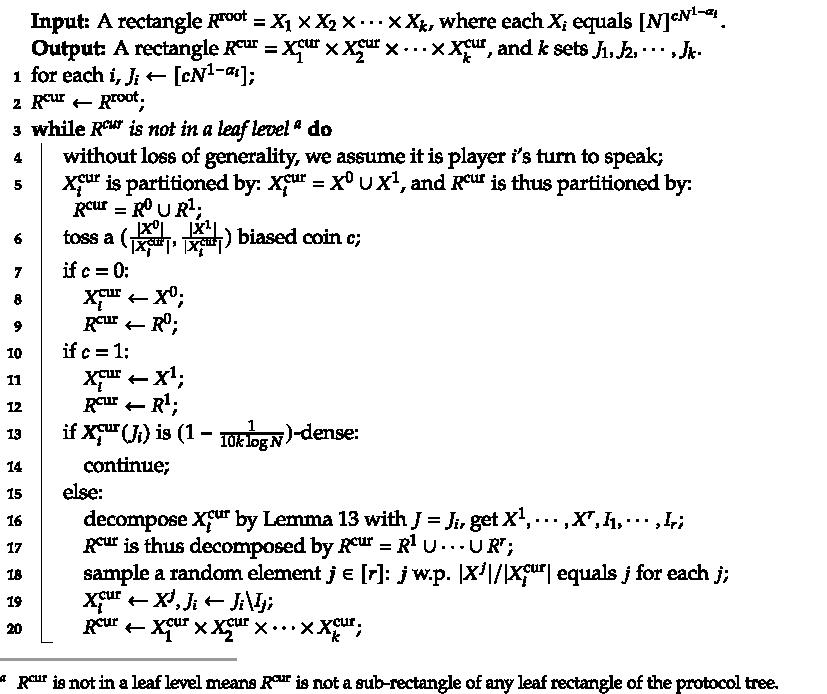
\includegraphics[width=\linewidth,height=0.78\textheight,keepaspectratio]{ccc2025-33-svg-01.pdf}\par




We use $R^{\text{cur}}$ to denote the current rectangle of the decomposition and sampling process. It begins with $R^{\text{cur}}=R^{\text{root}}$, and at each step $R^{\text{cur}}$ is partitioned into two subrectangles $R^{0},R^{1}$ by the protocol. Then, we replace $R^{\text{cur}}$ with $R^{0}$ or $R^{1}$ with probability $|R^{0}|/|R^{\text{cur}}|$ or $|R^{1}|/|R^{\text{cur}}|$ (which also equals to $|X^{0}|/|X_{i}^{\text{cur}}|$ or $|X^{1}|/|X_{i}^{\text{cur}}|$ as we defined in Algorithm 1), and reach a new rectangle. After reaching the new rectangle, the structured property of $R^{\text{cur}}$ may get destroyed, and our decomposition works here to maintain the structured property. We use the density-restoring partition (Lemma 13) to further decompose the current rectangle $R^{\text{cur}}$ into $r$ subrectangles $R^{\text{cur}}=R^{1}\cup R^{2}\cup\cdots\cup R^{r}$, and each $R^{j}$ is a structured rectangle. Again, we choose $R^{j}$ to be our next rectangle with probability $|R^{j}|/|R^{\text{cur}}|$, and do the process above recursively until reaching a leaf rectangle. As shown in the decomposition and sampling process, we eventually sample a structured rectangle in the leaf level with respect to its size.\par




\emph{Note that at some point of the random walk, the current rectangle $R^{\text{cur}}$ may not exist on the protocol tree since we do the density-restoring partition to further decompose the rectangles. However, every $R^{\text{cur}}$ that potentially appears in the random walk must be fully contained in a rectangle of the protocol tree. Thus, the protocol $\Pi$ also partitions $R^{\text{cur}}$ into two sub-rectangles if $R^{\text{cur}}$ is not in the leaf level of the protocol tree.}\par




Note that the output $R^{\text{cur}}$ of the process above is a random variable over rectangles. We define $\bm{R}^{\text{leaf}}$ to be the random variables over decomposed structured rectangles in the leaf level (not leaf rectangles of the protocol tree, but sub-rectangles of those leaves after decomposition) sampled by the process above, and $\bm{R}^{\text{leaf}}$ is associated with random sets $\bm{J}_{i}^{\text{leaf}}$s. For convenience, we define the support of $\bm{R}^{\text{leaf}}$ to be $\mathcal{R}^{\text{leaf}}$.
One may see the two important properties of the decomposition and sampling process:\par


\begin{itemize}


\item[] 
$\blacksquare$ 


Every rectangle $R\in\mathcal{R}^{\text{leaf}}$ is a structured rectangle;\par





\item[] 
$\blacksquare$ 


For a rectangle $R=X_{1}\times X_{2}\times\cdots\times X_{k}\in\mathcal{R}^{\text{leaf}}$, we have that\par


\[\begin{gathered}
\operatorname*{\mathbf{Pr}}[\bm{R}^{\text{leaf}}=R]=\prod_{i}\frac{|X_{i}|}{N^{cN^{1-\alpha_{i}}}}=\frac{|R|}{N^{c\sum_{i}N^{1-\alpha_{i}}}}.
\end{gathered}\]





\end{itemize}


The verification of the two properties is straightforward from the definition of our decomposition and sampling process. The first statement offers a structured property that makes it easier to analyze the rectangles. The second statement tells us that the probability that $\bm{R}^{\text{leaf}}=R$ equals the probability that the input lies in $R$. This is crucial in later bounding the accuracy of $\Pi$.\par




Next, we bound the accuracy of $\Pi$. For every structured rectangle $R=X_{1}\times X_{2}\times\cdots\times X_{k}\in\mathcal{R}^{\text{leaf}}$ associated with $J_{1},J_{2},\cdots,J_{k}$, we define $J_{i}^{c}$ as $[cN^{1-\alpha_{i}}]-J_{i}$, namely the fixed parts of $X_{i}$. Hence, for each $X_{i}$, it holds $\forall x\in X_{i},x(J_{i}^{c})=\beta_{i}$ since $R$ is a structured rectangle. We can then divide all the rectangles in $\mathcal{R}^{\text{leaf}}$ into two types:\par


\begin{enumerate}


\item[] 
1. 


$R$ is a \emph{bad} structured rectangle if $\cap_{i}\beta_{i}\neq\emptyset$;\par





\item[] 
2. 


$R$ is a \emph{good} structured rectangle if $\cap_{i}\beta_{i}=\emptyset$.\par





\end{enumerate}


Assume $R$ is a bad structured rectangle. Then, there exists a universal common element $a$\footnote{We can choose any element that lies in $\cap_{i}\beta_{i}$ here.} such that $a\in\cap_{i}x_{i}$ for any possible instance $(x_{1},x_{2},\cdots,x_{k})$ in $R$. The protocol is thus able to achieve perfect correctness by outputting $a$ when the input lies in $R$. Hence, we need to show with a low probability that $\bm{R}^{\text{leaf}}$ is a bad rectangle, namely the probability that the input lies in bad rectangles is small. To be more specific, we prove the following lemma:\par



% SOURCE-ID Thmtheorem17


\par\medskip\noindent\textbf{
\textbf{Lemma 17}\textbf{.}
}\par



\emph{If $\text{CC}(\Pi)\leq 0.0001N^{\sum_{i}{\alpha_{i}}-\mathop{\max}_{i}\{\alpha_{i}\}}/k$, it holds that
$\operatorname*{\mathbf{Pr}}_{R\sim\bm{R}^{\text{leaf}}}[R\text{ is bad}]\leq 0.05$.}\par



% END-SOURCE-ID Thmtheorem17



For those good structured rectangles, we show the following facts:
For a good structured rectangle, the protocol $\Pi$ cannot achieve high accuracy since there is no intersection on the fixed parts, while the other parts are dense.
Formally, we prove the following lemma:\par



% SOURCE-ID Thmtheorem18


\par\medskip\noindent\textbf{
\textbf{Lemma 18}\textbf{.}
}\par



\emph{For a good structured rectangle $R=X_{1}\times X_{2}\times\cdots\times X_{k}$,
it holds that for any $a\in[N]$,}\par


\[\begin{gathered}
\operatorname*{\mathbf{Pr}}[a\in\cap_{i}\bm{X}_{i}]\leq 0.05.
\end{gathered}\]



% END-SOURCE-ID Thmtheorem18



Combining the three lemmas above, we can easily prove Theorem 16.\par




\par\medskip\noindent\textbf{Proof of Theorem 16.}\par




We prove the theorem by showing that communication protocol $\Pi$ with $\text{CC}(\Pi)\leq 0.0001N^{\sum_{i}{\alpha_{i}}-\mathop{\max}_{i}\{\alpha_{i}\}}/k$ can achieve at most $0.1$ accuracy.\par




It is well known that a communication protocol $\Pi$ partitions the whole input domain into several leaf rectangles and assigns an answer to each leaf rectangle. With our decomposition and sampling process, original leaf rectangles are further decomposed into the two types of structured rectangles mentioned above. The accuracy of $\Pi$ comes from the following two parts:\par


\begin{enumerate}


\item[] 
1. 


The probability $\operatorname*{\mathbf{Pr}}[\bm{R}^{\text{leaf}}\text{ is bad}]=p_{1}$.\par





\item[] 
2. 


The probability that the protocol outputs the correct answer in a good structured rectangle is $p_{2}$.\par





\end{enumerate}


From Lemma 17 and 18, we know that $p_{1}\leq 0.05,p_{2}\leq 0.05$. By a union bound, the total accuracy is thus no more than $p_{1}+p_{2}\leq 0.1$ as desired.
$\blacktriangleleft$
It suffices to prove the two important lemmas above.\par






\par\medskip\noindent\textbf{
3.2 Proofs of Technical Lemmas}\par




We first prove Lemma 17 by the following round-by-round analysis.\par




\par\medskip\noindent\textbf{Proof of Lemma 17.}\par




Recall the decomposition process from line 4 to line 12. In each communication round, player $i$ sends one bit, and partitions $X_{i}^{\text{cur}}$ into two parts $X^{0},X^{1}$. Then, $X_{i}^{\text{cur}}$ is replaced by $X^{0}$ (or $X^{1}$) with probability $\frac{|X^{0}|}{|X_{i}^{\text{cur}}|}$ (or $\frac{|X^{1}|}{|X_{i}^{\text{cur}}|}$). In this process, the density function $\mathcal{D}(\bm{X}_{i}^{\text{cur}}(J_{i}))$ would increase since the size of $|X_{i}^{\text{cur}}|$ decreases. This contributes to the density function with an increment of:\par


\begin{itemize}


\item[] 
$\blacksquare$ 


$\log(\frac{|X_{i}^{\text{cur}}|}{|X^{0}|})$ with probability $|X^{0}|/|X_{i}^{\text{cur}}|$;\par





\item[] 
$\blacksquare$ 


$\log(\frac{|X_{i}^{\text{cur}}|}{|X^{1}|})$ with probability $|X^{1}|/|X_{i}^{\text{cur}}|$.\par





\end{itemize}


Thus, in expectation, the density function of $R^{\text{cur}}=X_{1}^{\text{cur}}\times X_{2}^{\text{cur}}\times\cdots\times X_{k}^{\text{cur}}$ after partitioning will increase\par


\[\begin{gathered}
\frac{|X^{0}|}{|X_{i}^{\text{cur}}|}\log\bigg{(}\frac{|X_{i}^{\text{cur}}|}{|X^{0}|}\bigg{)}+\frac{|X^{1}|}{|X_{i}^{\text{cur}}|}\log\bigg{(}\frac{|X_{i}^{\text{cur}}|}{|X^{1}|}\bigg{)}\leq 1,
\end{gathered}\]


where $|X_{i}^{\text{cur}}|$ denotes the size of $X_{i}^{\text{cur}}$ before partitioning. Furthermore, if $\bm{X}_{i}^{\text{cur}}(J_{i})$ is no longer $(1-\frac{1}{10k\log n})$-dense, we partition $X_{i}^{\text{cur}}$ by Lemma 13 and get $X_{i}^{\text{cur}}=X^{1}\cup X^{2}\cup\cdots\cup X^{r}$ and $I_{1}\cup I_{2}\cup\cdots\cup I_{r}$ with $X^{j}(I_{j})=\tau_{j}$ for all $j$. We use Lemma 13, where we take $\gamma=1-1/(10k\log N)$, and get:\par


\[\begin{gathered}
\mathcal{D}(\bm{X}^{j}(J_{i}-I_{i}))\leq\mathcal{D}(\bm{X}_{i}^{\text{cur}}(J_{i}))-(1-\gamma)|I_{j}|\log N+\gamma_{j}=\mathcal{D}(\bm{X}_{i}^{\text{cur}}(J_{i}))-\frac{|I_{j}|}{10k}+\delta_{j}.
\end{gathered}\]


Recall that $\delta_{j}:=\log(|X_{i}^{\text{cur}}|/|\cup_{p\geq j}X^{p}|)$ here. In the decomposition process, $X_{i}^{\text{cur}}$ is replaced with $X^{j}$ with probability $|X^{j}|/|X_{i}^{\text{cur}}|$. Hence, taking the expectation in one communication round, we have\par


\[\begin{gathered}
\mathbb{E}[\delta_{j}]=\sum_{j}\frac{|X^{j}|}{|X_{i}^{\text{cur}}|}\log(|X_{i}^{\text{cur}}|/|\cup_{p\geq j}X^{p}|)\leq\int_{0}^{1}\log\frac{1}{1-x}dx=1.
\end{gathered}\]


Thus, combining (1), (2) and (3) and taking expectations, we know that after $\text{CC}(\Pi)$ rounds of communication (where each round communicates exact one bit message), it holds:\par


\[\begin{gathered}
\mathbb{E}_{R\sim\bm{R}^{\text{leaf}}}[\mathcal{D}(R)]\leq 2\cdot\text{CC}(\Pi)-\frac{\mathbb{E}_{J_{1}\sim\bm{J}_{1}^{\text{leaf}},\cdots,J_{k}\sim\bm{J}_{k}^{\text{leaf}}}\bigg{[}\sum_{j=1}^{k}|J_{j}^{c}|\bigg{]}}{10k}.
\end{gathered}\]


Here, the $2\cdot\text{CC}(\Pi)$ comes from (1) and (3). We know that $\mathbb{E}_{R\sim\bm{R}^{\text{leaf}}}[\mathcal{D}(R)]\geq 0$ from definitions. Hence, we have\par


\[\begin{gathered}
\sum_{j=1}^{k}\mathbb{E}_{J_{j}\sim\bm{J}_{j}^{\text{leaf}}}[|J_{j}^{c}|]\leq 20k\cdot\text{CC}(\Pi).
\end{gathered}\]




We can bound the probability that the bad structured rectangle appears round by round. At each round of communication, if we choose $X^{j}$ to replace $X_{i}^{\text{cur}}$, then we will fix $|I_{j}|$ more positions for $X_{i}^{\text{cur}}$. We then consider the probability that this new fixed part contributes to forming a bad structured rectangle with future fixed positions.\par




Let $R^{j}=X_{1}^{\text{cur}}\times X_{2}^{\text{cur}}\times\cdots X^{j}\cdots\times X_{k}^{\text{cur}}$, for any $x=(x_{1}^{\text{cur}},x_{2}^{\text{cur}},\cdots,x^{j},\cdots,x_{k}^{\text{cur}})\in R^{j}$, we label it as a error term if $\exists a\in\tau_{j}$, $a\in\bigcap_{p\neq i}x_{p}^{\text{cur}}(J_{p})$ \footnote{ $\tau_{j}$ is a fixed subset of $[N]$ with size at most $|I_{j}|$ since $X^{j}$ is fixed on $I_{j}$. Input $x$ may be labeled many times during the decomposition process.}. By Lemma 15, for any $a\in\tau_{j}$,\par


\[\begin{gathered}
\operatorname*{\mathbf{Pr}}[a\in\bigcap_{p\neq i}\bm{X}_{p}^{\text{cur}}(J_{p})]\leq\frac{ec^{k-1}}{N^{(\sum_{p=1}^{k}\alpha_{p})-\alpha_{i}}}
\end{gathered}\]


By a union bound, the probability that error terms appear in $R^{j}$ is\par


\[\begin{gathered}
\operatorname*{\mathbf{Pr}}[\exists a\in\tau_{j},a\in\bigcap_{p\neq i}\bm{X}_{p}^{\text{cur}}(J_{p})]\leq\frac{|I_{j}|\cdot ec^{k-1}}{N^{(\sum_{p=1}^{k}\alpha_{p})-\alpha_{i}}}
\end{gathered}\]


Also, we know that the total number of fixed elements equals $\sum_{i=1}^{k}|J_{i}^{c}|$, which is identical to the summation of $|I_{j}|$ of every step, thus, the average probability of error terms at the end of the decomposition process is at most\par


\[\begin{gathered}
\frac{ec^{k-1}}{N^{(\sum_{i}\alpha_{i})-\mathop{\max}_{i}\{\alpha_{i}\}}}\cdot\sum_{i=1}^{k}\mathbb{E}_{J_{i}\sim\bm{J}_{i}^{\text{leaf}}}\big{[}|J_{i}^{c}|\big{]}.
\end{gathered}\]


We note that for any $R\in\mathcal{R}^{\text{leaf}}$, if $R$ is bad, then all instances $x\in R$ have been labeled as an error term in the decomposition process, together with (4), we have\par


\[\begin{gathered}
\operatorname*{\mathbf{Pr}}_{R\sim\bm{R}^{\text{leaf}}}[R\text{ is bad}]\leq\frac{ec^{k-1}}{N^{(\sum_{i}\alpha_{i})-\mathop{\max}_{i}\{\alpha_{i}\}}}\cdot\sum_{i=1}^{k}\mathbb{E}_{J_{i}\sim\bm{J}_{i}^{\text{leaf}}}\big{[}|J_{i}^{c}|\big{]}\leq 0.05.
\end{gathered}\]


The last inequality holds since $c=(1+2/k)$ and $\text{CC}(\Pi)\leq 0.0001N^{\sum_{i}{\alpha_{i}}-\mathop{\max}_{i}\{\alpha_{i}\}}/k$.
$\blacktriangleleft$
Next, we show that in the good structured rectangles, the protocol $\Pi$ cannot achieve large accuracy in finding the common element. This also comes from the structured properties of the rectangles:\par





\par\medskip\noindent\textbf{Proof of Lemma 18.}\par




Notice that we consider the rectangle $R=X_{1}\times X_{2}\times\cdots\times X_{k}$ associated with $J_{1},J_{2},\cdots J_{k}$ that has no common elements on fixed parts $J_{i}^{c}$. Thus, for any element $a\in[N]$, there exists at least a party $i$ which does not contain $a$ on its fixed part. Thus, we use Lemma 15 for $\bm{X}_{i}(J_{i})$ with $\ell=1$, and get\par


\[\begin{gathered}
\operatorname*{\mathbf{Pr}}[a\in\bm{X}_{i}]=\operatorname*{\mathbf{Pr}}[a\in\bm{X}_{i}(J_{i})]\leq ce/N^{\alpha_{i}}=o(1).\
\end{gathered}\]


$\blacktriangleleft$\par






\par\medskip\noindent\textbf{
3.3 Lower Bounds for Other Hardness Distributions}\par




In this section, we first establish a reduction from Bernoulli hardness distribution (hardness distribution 3) to hardness distribution 2 by the following lemma:\par



% SOURCE-ID Thmtheorem19


\par\medskip\noindent\textbf{
\textbf{Lemma 19}\textbf{.}
}\par



\emph{If a communication protocol $\Pi$ that solves set-intersection under hardness distribution 3 with accuracy $\epsilon$, there exists parameters $c_{1},\cdots,c_{k}$ with each $1-1/k\leq c_{i}\leq 1+1/k$ for hardness distribution 2 so that $\Pi$ can find set intersection under this distribution with accuracy $\epsilon-2k\mathop{\exp}(-\frac{N^{1-\mathop{\max}_{i}\{\alpha_{i}\}}}{3k^{2}})$, which is bigger than $\epsilon-0.01$ when $N^{1-\mathop{\max}_{i}\{\alpha_{i}\}}\geq 100k^{2}\log k$.}\par



% END-SOURCE-ID Thmtheorem19



\par\medskip\noindent\textbf{Proof.}\par




We first use Chernoff bound to bound the probability of the size of set $S_{i}$ of each player $i$ exceeding $(1+1/k)\cdot N^{1-\alpha_{i}}$ or less than $(1-1/k)\cdot N^{1-\alpha_{i}}$ under the hardness distribution 3:\par


\[\begin{gathered}
\displaystyle\operatorname*{\mathbf{Pr}}[||S_{i}|-N^{1-\alpha_{i}}|>1/k\cdot N^{1-\alpha_{i}}]\leq 2\exp\bigg{(}-\frac{N^{1-\alpha_{i}}}{3k^{2}}\bigg{)}.
\end{gathered}\]


We use $A$ to denote the event that $\exists i,||X_{i}|-N^{1-\alpha_{i}}|>1/k\cdot N^{1-\alpha_{i}}$. Then, by a union bound, we know that:\par


\[\begin{gathered}
\operatorname*{\mathbf{Pr}}[A]\leq 2k\cdot\exp\bigg{(}-\frac{N^{1-\mathop{\max}_{i}\{\alpha_{i}\}}}{3k^{2}}\bigg{)}.
\end{gathered}\]


Then, condition on $\neg A$, we have the success probability of $\Pi$ in finding set intersection under hardness distribution 3 is bigger than $\epsilon-2k\cdot\exp\bigg{(}-\frac{N^{1-\mathop{\max}_{i}\{\alpha_{i}\}}}{3k^{2}}\bigg{)}$. Furthermore, condition on $\neg A$, the hardness distribution 3 can be represented by a combination of product distributions:\par


\[\begin{gathered}
\sum_{c_{1},c_{2},\cdots,c_{k}}\sigma(c_{1},c_{2},\cdots,c_{k})D_{c_{1},c_{2},\cdots,c_{k}},
\end{gathered}\]


where $D_{c_{1},c_{2},\cdots,c_{k}}$ denotes the hardness distribution 2 with parameters $c_{1},c_{2},\cdots,c_{k}$. Then, the lemma follows from an averaging argument.
$\blacktriangleleft$
It suffices to construct a reduction from hardness distribution 2 to hardness distribution 1.\par



% SOURCE-ID Thmtheorem20


\par\medskip\noindent\textbf{
\textbf{Lemma 20}\textbf{.}
}\par



\emph{If there exists a communication protocol $\Pi$ with communication complexity $C$ which solves set-intersection under hardness distribution 2 with accuracy $\epsilon$, there exists a communication protocol $\Pi^{\prime}$ with communication complexity $C$ which solves set-intersection under hardness distribution 1 with accuracy $\epsilon-0.05$ when $k^{2}N^{-\min_{i}\{\alpha_{i}\}}\leq\frac{1}{100}$ holds.}\par



% END-SOURCE-ID Thmtheorem20




\par\medskip\noindent\textbf{Proof.}\par




We construct the communication protocol $\Pi^{\prime}$ as follows:\par


\begin{enumerate}


\item[] 
1. 


For each player $i$, remove the duplicate elements of its input and get a $S_{i}\subseteq[N]$.\par





\item[] 
2. 


Randomly sample $c_{i}N^{1-\alpha_{i}}$ elements from $S_{i}$, $\Pi^{\prime}$ fail if $|Y_{i}|<c_{i}N^{1-\alpha_{i}}$.\par





\item[] 
3. 


Run the communication protocol $\Pi$ on $Y_{i}$s to find intersection.\par





\end{enumerate}


We know that the successful probability of $\Pi^{\prime}$ under hardness distribution 1 is bigger than\par


\[\begin{gathered}
\epsilon-\operatorname*{\mathbf{Pr}}[\Pi^{\prime}\text{ fail at step 2}].
\end{gathered}\]


It suffices to bound $\operatorname*{\mathbf{Pr}}[\Pi^{\prime}\text{ fail at step 2}]$. From the union bound, we have:\par


\[\begin{gathered}
\displaystyle\operatorname*{\mathbf{Pr}}[\Pi^{\prime}\text{ fail at step 2}] \displaystyle\leq k\cdot\operatorname*{\mathbf{Pr}}[|S_{i}|<c_{i}N^{1-\alpha_{i}}] \\
\displaystyle\leq k\cdot\operatorname*{\mathbf{Pr}}[\#\text{repeated elements in $S_{i}$}>(c-c_{i})N^{1-\alpha_{i}}].
\end{gathered}\]


We know that\par


\[\begin{gathered}
\mathbb{E}[\#\text{repeated elements}]=cN^{1-\alpha_{i}}\bigg{(}1-(1-1/N)^{cN^{1-\alpha_{i}}-1}\bigg{)}\leq c^{2}N^{1-2\alpha_{i}}.
\end{gathered}\]


From Markov’s Inequality, we have\par


\[\begin{gathered}
\operatorname*{\mathbf{Pr}}[\#\text{repeated elements}>(c-c_{i})N^{1-\alpha_{i}}]\leq\mathbb{E}[\#\text{repeated elements}]/(c-c_{i})N^{1-\alpha_{i}}\leq kc^{2}N^{-\alpha_{i}}.
\end{gathered}\]


If $kN^{-\alpha_{i}}\leq\frac{1}{100k}$ holds, which is guaranteed by the constraints, $\operatorname*{\mathbf{Pr}}[\Pi^{\prime}\text{ fail at step 2}]\leq 0.05$ also holds. This concludes the lemma.
$\blacktriangleleft$\par






\par\medskip\noindent\textbf{
3.4 Efficient Protocols for the Hardness Distribution}\par




In this section, we first explain an efficient protocol for the hardness distribution 3, where we use $D_{3}$ to denote the distribution, showing that our lower bound result is almost tight for this distribution. Also, this protocol can be easily extended to some more general product distributions sharing \emph{"similarities"} with the Bernoulli product distribution.
Formally, we prove:\par



% SOURCE-ID Thmtheorem21


\par\medskip\noindent\textbf{
\textbf{Theorem 21}\textbf{.}
}\par



\emph{There is a protocol $\Pi$, which solves the hardness distribution 3, with $\text{Acc}_{\Pi}(D_{3})\geq 0.1$ and}\par


\[\begin{gathered}
\text{CC}(\Pi)=O(N^{\sum_{i}\alpha_{i}-\mathop{\max}_{i}\{\alpha_{i}\}}\log N).
\end{gathered}\]




\emph{Furthermore, this protocol can be extended to more general distributions. Let $D$ be any distribution that satisfies the following properties:}\par


\begin{enumerate}


\item[] 
1. 


\emph{each party holds a set of size }$\Theta(N^{1-\alpha_{i}})$\emph{;}\par





\item[] 
2. 


\emph{the size of intersecting part of all parties is }$\Omega(N^{1-\sum_{i}\alpha_{i}})$\emph{;}\par





\end{enumerate}


\emph{there exists a protocol $\Pi^{\prime}$ with $O(k\log N\cdot N^{\sum_{i}\alpha_{i}-\mathop{\max}_{i}\{\alpha_{i}\}})$ communication cost that achieves $\Omega(1)$ accuracy under $D$.}\par



% END-SOURCE-ID Thmtheorem21



\par\medskip\noindent\textbf{Proof.}\par




To begin with, we first propose an efficient protocol to solve $D_{3}$.
Without loss of generality, we assume $\alpha_{1}\geq\alpha_{2}\geq\cdots\geq\alpha_{k}$ and each party $i$ gets a subset $S_{i}\subseteq[N]$. Then, the communication protocol $\Pi$ proceeds as follows:\par


\begin{enumerate}


\item[] 
1. 


The first party uniformly and randomly picks $\mathop{\min}\{|S_{1}|,N^{\sum_{i}\alpha_{i}-\mathop{\max}_{i}\{\alpha_{i}\}}\}$ elements from $S_{1}$ and sends them, denoted by $M_{1}$, to the second party.\par





\item[] 
2. 


The second party receives the message $M_{1}$ from the first one, and sends $M_{2}:=M_{1}\bigcap S_{2}$ to the third party.\par





\item[] 
3. 


The process goes on, and the last party computes $M_{k-1}\bigcap S_{k}$. If it is not empty, the last party outputs any element in it. Otherwise, the protocol fails.\par





\end{enumerate}


Then, we bound $\text{Acc}_{\Pi}(D_{3})$ and its communication complexity to show $\Pi$ is highly efficient. From the definitions, we know that\par


\[\begin{gathered}
\text{Acc}_{\Pi}(D_{3})=\operatorname*{\mathbf{Pr}}[M_{1}\cap S_{2}\cap\cdots\cap S_{k}\neq\emptyset].
\end{gathered}\]


Also, we have that\par


\[\begin{gathered}
\operatorname*{\mathbf{Pr}}[M_{1}\cap S_{2}\cap\cdots\cap S_{k}\neq\emptyset||M_{1}|=m]=1-\bigg{(}1-\frac{1}{N^{\sum_{i}\alpha_{i}-\mathop{\max}_{i}\{\alpha_{i}\}}}\bigg{)}^{m}\geq\frac{m}{e\cdot N^{\sum_{i}\alpha_{i}-\mathop{\max}_{i}\{\alpha_{i}\}}}.
\end{gathered}\]


The last inequality holds since $m\leq N^{\sum_{i}\alpha_{i}-\mathop{\max}_{i}\{\alpha_{i}\}}$. From Chernoff bound, we know that the probability that $\operatorname*{\mathbf{Pr}}\big{[}|M_{1}|\leq N^{\sum_{i}\alpha_{i}-\mathop{\max}_{i}\{\alpha_{i}\}}/2\big{]}\leq e^{-N^{1-\alpha_{1}}/12}\leq e^{-10k^{3}}$. The last inequality is from the constraint of $k\leq 0.1\cdot\min\{N^{\min_{i}\{\alpha_{i}\}/2},N^{(1-\max_{i}\{\alpha_{i}\})/3}\}$. Furthermore, when\par


\[\begin{gathered}
|M_{1}|\geq N^{\sum_{i}\alpha_{i}-\mathop{\max}_{i}\{\alpha_{i}\}}/2,
\end{gathered}\]


it holds that\par


\[\begin{gathered}
\operatorname*{\mathbf{Pr}}[M_{1}\cap S_{2}\cap\cdots\cap S_{k}\neq\emptyset||M_{1}|=m]\geq\frac{1}{2e}.
\end{gathered}\]


Combining the facts above, we have $\text{Acc}_{\Pi}(D_{3})\geq\frac{1}{2e}\big{(}1-e^{-10k^{3}}\big{)}\geq 0.1$.\par




On the other hand, we bound the communication complexity by bounding the expected size of $|M_{i}|$. $\mathbb{E}[|M_{1}|]\leq N^{\sum_{i}\alpha_{i}-\mathop{\max}_{i}\{\alpha_{i}\}}\log
N$ holds from definitions. Furthermore, we have\par


\[\begin{gathered}
\mathbb{E}[|M_{i}|]\leq\mathbb{E}[|M_{i-1}|]\cdot N^{-\alpha_{i}}.
\end{gathered}\]


Then, $\mathbb{E}[\sum_{i}M_{i}]\leq O(N^{\sum_{i}\alpha_{i}-\mathop{\max}_{i}\{\alpha_{i}\}}\log n)$ follows by $N^{-\alpha_{i}}\leq N^{\min_{i}\{\alpha_{i}\}}\leq 1/2$. This concludes the first statement.\par




Next, we slightly change the protocol above to match the second statement. The protocol $\Pi^{\prime}$ proceeds as follows:\par


\begin{enumerate}


\item[] 
1. 


The first party uniformly and randomly picks $\Theta(N^{\sum_{i}\alpha_{i}-\mathop{\max}_{i}\{\alpha_{i}\}})$ elements from $S_{1}$ and sends them, denoted by $M_{1}$, to the second party.\par





\item[] 
2. 


The second party receives the message $M_{1}$ from the first one, and sends $M_{2}:=M_{1}\bigcap S_{2}$ to the third party.\par





\item[] 
3. 


The process goes on, and the last party computes $M_{k-1}\bigcap S_{k}$. If it is not empty, the last party outputs any element in it.\par





\end{enumerate}




Obviously, the communication complexity of this protocol $\Pi^{\prime}$ is $O(k\log n\cdot N^{\sum_{i}\alpha_{i}-\mathop{\max}_{i}\{\alpha_{i}\}})$. Also, we know the accuracy is bigger than\par


\[\begin{gathered}
\Omega\bigg{(}1-(1-\frac{\Omega(N^{1-\sum_{i}\alpha_{i}})}{|S_{1}|})^{\Theta(N^{\sum_{i}\alpha_{i}-\mathop{\max}_{i}\{\alpha_{i}\}})}\bigg{)}=\Omega(1).\
\end{gathered}\]


$\blacktriangleleft$
Thus, our lower bounds show that those trivial protocols are nearly optimal.\par







\par\medskip\noindent\textbf{
4 Lower Bounds for Chained Index}\par




Recall that in the Chained Index problem, the player $i$ receives an input $z_{i}=(\sigma_{i},x_{i})\in[n]\times\{0,1\}^{n}$. The players aim to compute $x_{k-1}(\sigma_{k})$ through a one-way communication. In this section, we show an improved lower bound for the Chained Index problem. In light of Yao’s principle, we consider the following hard distribution.\par



The distribution $\chi_{k}$.\par


\begin{enumerate}


\item[] 
1. 


Uniformly sample $\sigma_{1},...,\sigma_{k}\in[n]$.\par





\item[] 
2. 


Sample $(x_{1},\dots,x_{k})\sim(\left\{0,1\right\}^{n})^{k}$ conditioned on
$x_{1}(\sigma_{2})=\cdots=x_{k-1}(\sigma_{k})$.\par





\item[] 
3. 


Output $z=(z_{1},\dots,z_{k})$ where $z_{i}=(\sigma_{i},x_{i})$ for every $i\in[k]$.\par





\end{enumerate}



For a subset $R\subseteq([n]\times\left\{0,1\right\}^{n})^{k}$, define the weight of $R$ under $\chi_{k}$ as\par


\[\begin{gathered}
\chi_{k}(R)\stackrel{{\scriptstyle\mathsf{def}}}{{=}}\operatorname*{\mathbf{Pr}}_{z\sim\chi_{k}}\left[z\in R\right]=\frac{\#{\left\{((\sigma_{1},x_{1}),\dots,(\sigma_{k},x_{k}))\in R:x_{1}(\sigma_{2})=\cdots=x_{k-1}(\sigma_{k})\right\}}}{n^{k}\cdot 2^{(k-1)(n-1)+n+1}}.
\end{gathered}\]


We prove the following lower bound.
We say a one-way $k$-party protocol has \emph{signature} $(C_{1},\dots,C_{k})$ if, for each $i\in[k]$, the $i$-th party sends at most $C_{i}$ bits (on all inputs).\par



% SOURCE-ID Thmtheorem22


\par\medskip\noindent\textbf{
\textbf{Theorem 22}\textbf{.}
}\par



\emph{Let $\varepsilon\in(0,\nicefrac{{1}}{{4}}]$ be a constant.
Let $\Pi$ be a protocol for the $k$-party chained index problem with signature $(C_{1},\dots,C_{k})$.
If $\Pi$ has $2\varepsilon$ advantage, i.e.,}\par


\[\begin{gathered}
\operatorname*{\mathbf{Pr}}_{z=(\sigma_{1},x_{1},\dots,\sigma_{k},x_{k})\sim\chi_{k}}\left[\Pi(z)=x_{k-1}(\sigma_{k})\right]\geq\frac{1}{2}+2\varepsilon.
\end{gathered}\]


\emph{Then $\sum_{t=1}^{k}C_{t}\geq\max\left\{\frac{1}{32}\varepsilon^{2}n/k,\frac{1}{8}\varepsilon\sqrt{n}\right\}=\Omega(n/k+\sqrt{n})$.}\par



% END-SOURCE-ID Thmtheorem22



We use a decomposition and sampling process $\mathsf{DS}$, as shown in Algorithm 2, in our analysis.
$\mathsf{DS}$ takes as input a protocol $\Pi$,
and samples a rectangle $R$ that is contained in $\Pi_{v}$ for some leaf node $v$.
Our proof proceeds in two steps:\par


\begin{enumerate}


\item[] 
1. 


Section 4.1 shows that the accuracy of $\Pi$ is captured by a quantity called \emph{average fixed size}, which is a natural quantity that arises in the running of $\mathsf{DS}$.\par





\item[] 
2. 


Section 4.2 proves that the average fixed size can be bounded from above by $O(k\cdot\mathrm{CC}(\Pi))$. Consequently, if $\Pi$ enjoys high accuracy, we get a lower bound of $\mathrm{CC}(\Pi)$.\par





\end{enumerate}




We first recall some basic definitions.\par




\par\medskip\noindent\textbf{
$k$-party one-way protocols}\par




A deterministic $k$-party one-way communication protocol $\Pi$ is specified by a rooted binary tree.
For every internal vertex $v$,\par


\begin{itemize}


\item[] 
$\blacksquare$ 


it has 2 children, denoted by $\Pi(v,0)$ and $\Pi(v,1)$;\par





\item[] 
$\blacksquare$ 


$v$ is owned by some party – we denote the owner by $\mathsf{owner}(v)\in[k]$;\par





\item[] 
$\blacksquare$ 


every leaf node specifies an output.\par





\end{itemize}


Starting from the root,
the owner of the current node $\mathsf{cur}$ partitions its input space into two parts $X_{0}$ and $X_{1}$, and sets the current node to $\Pi(\mathsf{cur},b)$ if its input belongs to $X_{b}$.\par




The \emph{communication complexity} of $\Pi$, denoted by $\mathrm{CC}(\Pi)$, is the depth of the tree.
On a path from root to some leaf, each time the owner switches, we call it a new \emph{round}; in a one-way protocol, the label of the owner is non-decreasing.\par



% SOURCE-ID Thmtheorem23


\par\medskip\noindent\textbf{
\textbf{Fact 23}\textbf{.}
}\par



\emph{The set of all inputs that lead to an internal vertex $v$ is a rectangle, denoted by $\Pi_{v}=X_{1}\times\cdots\times X_{k}$.}\par



% END-SOURCE-ID Thmtheorem23




\par\medskip\noindent\textbf{Normalized protocols}\par




We normalized a protocol $\Pi$ as follows so as to make it defined on all inputs, including those not in $\mathrm{supp}(\chi_{k})$.
For the $i$-th party, given input $(\sigma_{i},x_{i})\in[n]\times\left\{0,1\right\}^{n}$ and previous transcripts $\mathsf{trans}$,
output $0$ if the input is \emph{invalid}, i.e., given $\mathsf{trans}$,
there is no input in $\mathrm{supp}(\chi_{k})$ matches $x_{i}$.
Otherwise, the $i$-th party outputs $1$ and proceeds as $\Pi$.
Clearly, by normalizing, we communicate $k$ more bits.\par


\textbf{Algorithm 2}  Decomposition and Sampling Process $\mathsf{DS}$.

\par\noindent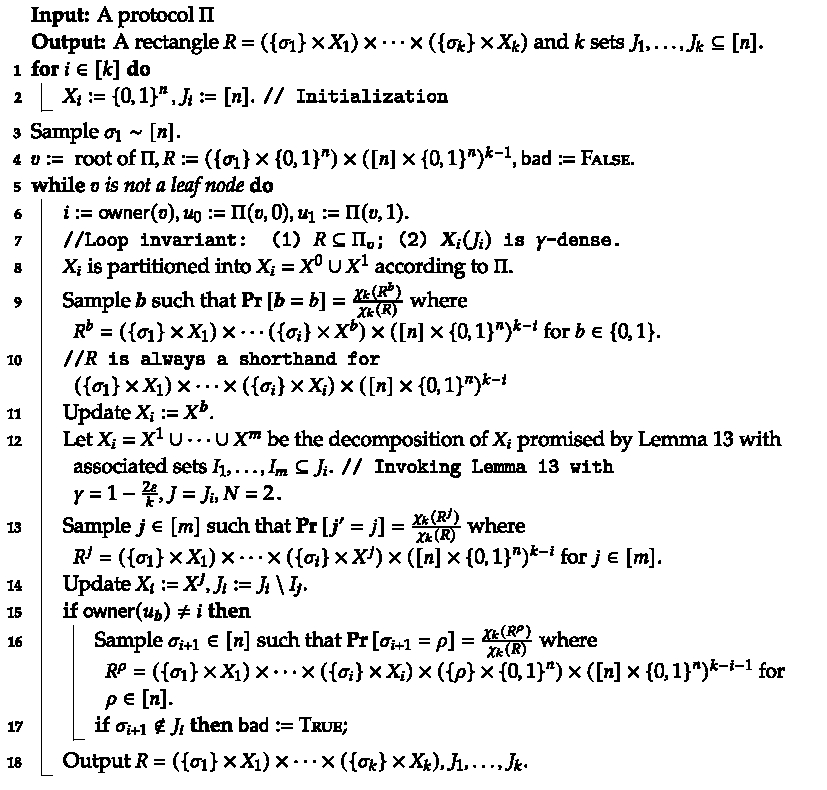
\includegraphics[width=\linewidth,height=0.78\textheight,keepaspectratio]{ccc2025-33-svg-02.pdf}\par



% SOURCE-ID Thmtheorem24


\par\medskip\noindent\textbf{
\textbf{Lemma 24}\textbf{ }(Loop invariant)\textbf{.}
}\par



\emph{After each iteration in algorithm 2,}\par


\begin{itemize}


\item[] 
$\blacksquare$ 


$R\subseteq\Pi_{v}$\emph{;}\par





\item[] 
$\blacksquare$ 


\emph{for all }$i\in[k]$\emph{, }$\bm{X}_{i}(J_{i})$\emph{ is }$\gamma$\emph{-dense;}\par





\item[] 
$\blacksquare$ 


\emph{for all }$i\in[k]$\emph{, there exists }$\alpha_{i}\in\left\{0,1\right\}^{\overline{J_{i}}}$\emph{ such that }$x(\overline{J_{i}})=\alpha_{i}$\emph{ for all }$x\in X_{i}$\emph{.}\par





\end{itemize}



% END-SOURCE-ID Thmtheorem24



\par\medskip\noindent\textbf{Proof.}\par




The first item is true because every time $v$ is updated,
$R$ is updated accordingly to a sub-rectangle of $\Pi_{v}$ and updating $R$ into its sub-rectangles does not violate this condition.\par




Since we applied density restoring partition at the end of each iteration, the second and the third items are guaranteed by Lemma 13 and the way that $X_{i},J_{i}$ are updated.
$\blacktriangleleft$\par






\par\medskip\noindent\textbf{
4.1 Relating Accuracy and Average Fixed Size}\par




As shown in Lemma 24, during the execution of $\mathsf{DS}(\Pi)$, for every $i\in[k]$, the set $X_{i}$ is “fixed” on $\overline{J_{i}}$ in the sense that all strings in $X_{i}$ share the same value on coordinates in $\overline{J_{i}}$. So we call the expected size of $|\overline{J_{i}}|$ \emph{average fixed size}. However, in order to relate the accuracy of $\Pi$ to average fixed size, we need to consider the expectation of $|\overline{J_{i}}|$ in a slightly different distribution.\par



% SOURCE-ID Thmtheorem25


\par\medskip\noindent\textbf{
\textbf{Definition 25}\textbf{ }(Average fixed size)\textbf{.}
}\par



\emph{Let $\mathcal{U}_{k}$ denote the uniform distribution over the input space $([n]\times\left\{0,1\right\}^{n})^{k}$.
Let $t\in[k]$ and consider the following process, denoted by $\mathsf{Unif}_{t}(\Pi)$:}\par


\begin{enumerate}


\item[] 
1. 


\emph{run }$\mathsf{DS}(\Pi)$\emph{ until the }$t$\emph{-th round;}\par





\item[] 
2. 


\emph{continue running }$\mathsf{DS}$\emph{ with }$\chi_{k}$\emph{ replaced by }$\mathcal{U}_{k}$\emph{ in the execution of Line }9\emph{, Line }13\emph{, and Line }16\emph{;}\par





\item[] 
3. 


\emph{upon entering the }$(t+1)$\emph{-th round (i.e., until Line }17\emph{ is reached with }$i=t$\emph{), return }$J_{t}$\emph{.}\par





\end{enumerate}


\emph{The average fixed size of the $t$-th party is defined as
$\operatorname*{\mathbf{E}}_{J_{t}\sim\mathsf{Unif}_{t}(\Pi)}\left[|\overline{J_{t}}|\right].$}\par



% END-SOURCE-ID Thmtheorem25


% SOURCE-ID Thmtheorem26


\par\medskip\noindent\textbf{
\textbf{Lemma 26}\textbf{ }(Relating accuracy and average fixed size)\textbf{.}
}\par



\emph{Assume that $\gamma\geq\log\left[1+\left(\frac{1-2\varepsilon}{1+2\varepsilon}\right)^{1/k}\right]$.
Then}\par


\[\begin{gathered}
\operatorname*{\mathbf{Pr}}_{z=(\sigma_{1},x_{1},\dots,\sigma_{k},x_{k})\sim\chi_{k}}\left[\Pi(z)=x_{k-1}(\sigma_{k})\right]\leq\frac{1}{2}+\varepsilon+\frac{2}{n}\cdot\sum_{t=1}^{k}\operatorname*{\mathbf{E}}_{J_{t}\sim\mathsf{Unif}_{t}(\Pi)}\left[|\overline{J_{t}}|\right].
\end{gathered}\]



% END-SOURCE-ID Thmtheorem26


% SOURCE-ID Thmtheorem27


\par\medskip\noindent\textbf{
$\blacktriangleright$ Remark 27.
}\par



$\gamma\stackrel{{\scriptstyle\mathsf{def}}}{{=}}1-\frac{2\varepsilon}{k}$\emph{ satisfies the condition.
Indeed,}\par


\[\begin{gathered}
\log\left[1+\left(\frac{1-2\varepsilon}{1+2\varepsilon}\right)^{1/k}\right]\leq\left(\frac{1-2\varepsilon}{1+2\varepsilon}\right)^{1/k}\leq 1-\frac{1}{k}\cdot\frac{4\varepsilon}{1+2\varepsilon}\leq 1-\frac{2\varepsilon}{k},
\end{gathered}\]


\emph{where the first inequality is by $\log(1+x)\leq x$, and the second is by $(1-x)^{r}\leq 1-rx$ for $x\in(-1,0)$ and $r\in(0,1)$.}\par



% END-SOURCE-ID Thmtheorem27



The proof of the lemma is obtained through the following two lemmas.
The first lemma readily says that conditioned on the flag $\mathsf{bad}$ is not raised, $\Pi$ has little advantage in the rectangle $R$ output by $\mathsf{DS}(\Pi)$.
The second lemma shows the probability that the flag is raised is bounded in terms of the average fixed size.\par



% SOURCE-ID Thmtheorem28


\par\medskip\noindent\textbf{
\textbf{Lemma 28}\textbf{.}
}\par



\emph{If $\mathsf{DS}(\Pi)$ outputs $(R,J_{1},\dots,J_{k})$ and $\mathsf{bad}=\textsc{False}$ in the end, then}\par


\[\begin{gathered}
\operatorname*{\mathbf{Pr}}_{z=(\rho_{1},x_{1},\dots,\rho_{k},x_{k})\sim R}\left[\Pi(z)=x_{k-1}(\rho_{k})|x_{1}(\rho_{2})=\cdots=x_{k-1}(\rho_{k})\right]\leq\frac{1}{2}+\varepsilon.
\end{gathered}\]



% END-SOURCE-ID Thmtheorem28


% SOURCE-ID Thmtheorem29


\par\medskip\noindent\textbf{
\textbf{Lemma 29}\textbf{.}
}\par



$\operatorname*{\mathbf{Pr}}_{\mathsf{DS}(\Pi)}\left[\mathsf{bad}=\textsc{True}\right]\leq\frac{2}{n}\cdot\sum_{t=1}^{k}\operatorname*{\mathbf{E}}_{J_{t}\sim\mathsf{Unif}_{t}(\Pi)}\left[|\overline{J_{t}}|\right].$\emph{}\par



% END-SOURCE-ID Thmtheorem29



Next, we first prove Lemma 26 using the above two lemmas.\par




\par\medskip\noindent\textbf{Proof of Lemma 26.}\par




Note that in the running of $\mathsf{DS}(\Pi)$,
we first sample $\sigma_{1},\dots,\sigma_{k}\sim[n]$ and then
always update $R$ to a randomly chosen rectangle; the probability of each rectangle being chosen is proportional to its weight under $\chi_{k}$.
Consequently,\par




\[\begin{gathered}
\displaystyle\quad\operatorname*{\mathbf{Pr}}_{z=(\sigma_{1},x_{1},\dots,\sigma_{k},x_{k})\sim\chi_{k}}\left[\Pi(z)=x_{k-1}(\sigma_{k})\right] \\
\displaystyle=\operatorname*{\mathbf{Pr}}_{\begin{subarray}{c}(R,J_{1},\dots,J_{k})\sim\mathsf{DS}(\Pi)\\
(\sigma_{1},x_{1},\dots,\sigma_{k},x_{k})\sim R\end{subarray}}\left[\Pi(z)=x_{k-1}(\sigma_{k})\;\middle|\;x_{1}(\sigma_{2})=\cdots=x_{k-1}(\sigma_{k})\right] \\
\displaystyle\leq\operatorname*{\mathbf{Pr}}_{\mathsf{DS}(\Pi)}\left[\mathsf{bad}=\textsc{True}\right]+\operatorname*{\mathbf{Pr}}_{\begin{subarray}{c}(R,J_{1},\dots,J_{k})\sim\mathsf{DS}(\Pi)\\
z=(\sigma_{1},x_{1},\dots,\sigma_{k},x_{k})\sim R\end{subarray}}\left[\Pi(z)=x_{k-1}(\sigma_{k})|x_{1}(\sigma_{2})=\cdots=x_{k-1}(\sigma_{k})\land\mathsf{bad}=\textsc{False}\right] \\
\displaystyle\leq\frac{1}{2}+\varepsilon+\frac{2}{n}\cdot\sum_{t=1}^{k}\operatorname*{\mathbf{E}}_{J_{t}\sim\mathsf{Unif}_{t}(\Pi)}\left[|\overline{J_{t}}|\right].
\end{gathered}\]


where the last step is by Lemma 28 and Lemma 29.
$\blacktriangleleft$\par




It remains to prove the two lemmas.\par





\par\medskip\noindent\textbf{Proof of Lemma 28.}\par




Say $R=(\left\{\sigma_{1}\right\}\times X_{1})\times\cdots\times(\left\{\sigma_{k}\right\}\times X_{k})$.
Since $\mathsf{bad}=\textsc{False}$ in the end,
we have $\sigma_{i+1}\in J_{i}$ for all $i\in[k-1]$.
By Lemma 24, we have $\text{H}_{\infty}(\bm{X}_{i}(\sigma_{i+1}))\geq\gamma$ for all $i$.
Since $R$ is contained in some leaf node of $\Pi$,
$\Pi$ output the same answer in $R$, say $b^{*}\in\left\{0,1\right\}$.
Note that for $b\in\left\{0,1\right\}$,\par


\[\begin{gathered}
\operatorname*{\mathbf{Pr}}_{z=(\rho_{1},x_{1},\dots,\rho_{k},x_{k})\sim R}\left[x_{1}(\rho_{2})=\cdots=x_{k-1}(\rho_{k})=b\right]=\prod_{i\in[k-1]}\operatorname*{\mathbf{Pr}}_{x_{i}\sim X_{i}}\left[x_{i}(\sigma_{i+1})=b\right],
\end{gathered}\]


since we must have $\rho_{i}=\sigma_{i}$.
Write $p_{i}\stackrel{{\scriptstyle\mathsf{def}}}{{=}}\operatorname*{\mathbf{Pr}}_{x^{i}\sim X^{i}}\left[x^{i}(\sigma_{i})=b^{*}\right]$.
Then we have\par




\[\begin{gathered}
\displaystyle\quad\operatorname*{\mathbf{Pr}}_{z=(\rho_{1},x_{1},\dots,\rho_{k},x_{k})\sim R}\left[\Pi(z)=x_{k-1}(\rho_{k})|x_{1}(\rho_{2})=\cdots=x_{k-1}(\rho_{k})\right] \\
\displaystyle=\operatorname*{\mathbf{Pr}}_{z=(\rho_{1},x_{1},\dots,\rho_{k},x_{k})\sim R}\left[x_{1}(\rho_{2})=\cdots=x_{k-1}(\rho_{k})=b^{*}|x_{1}(\rho_{2})=\cdots=x_{k-1}(\rho_{k})\right] \\
\displaystyle=\operatorname*{\mathbf{Pr}}_{z=(\rho_{1},x_{1},\dots,\rho_{k},x_{k})\sim R}\left[x_{1}(\sigma_{2})=\cdots=x_{k-1}(\sigma_{k})=b^{*}\right]/\operatorname*{\mathbf{Pr}}_{z=(\rho_{1},x_{1},\dots,\rho_{k},x_{k})\sim R}\left[x_{1}(\sigma_{2})=\cdots=x_{k-1}(\sigma_{k})\right] \\
\displaystyle=\frac{\prod_{i\in[k]}p_{i}}{\prod_{i\in[k]}p_{i}+\prod_{i\in[k]}(1-p_{i})}=\frac{1}{1+\prod_{i\in[k]}(1/p_{i}-1)}.
\end{gathered}\]


Since $\text{H}_{\infty}(\bm{X}_{i}(\sigma_{i+1}))\geq\gamma$ for all $i$, we have $p_{i}\in[1-2^{-\gamma},2^{-\gamma}]$, which implies\par


\[\begin{gathered}
\frac{1}{1+\prod_{i\in[k]}(1/p_{i}-1)}\leq\frac{1}{1+(2^{\gamma}-1)^{k}}.
\end{gathered}\]


Since we assumed $\gamma\geq\log\left[1+\left(\frac{1-2\varepsilon}{1+2\varepsilon}\right)^{1/k}\right]$, it holds that $\frac{1}{1+(2^{\gamma}-1)^{k}}\leq\frac{1}{2}+\varepsilon$, concluding the proof.
$\blacktriangleleft$\par





\par\medskip\noindent\textbf{Proof of Lemma 29.}\par




Let $\mathcal{B}_{t}$ denote the event that the flag $\mathsf{bad}$ is raised when $i=t$ (i.e., when the $i$-th round ends) for the first time.
Clearly,
$\operatorname*{\mathbf{Pr}}\left[\mathsf{bad}=\textsc{True}\right]=\sum_{t=1}^{k-1}\operatorname*{\mathbf{Pr}}\left[\mathcal{B}_{t}\right].$
It suffices to show $\operatorname*{\mathbf{Pr}}\left[\mathcal{B}_{t}\right]\leq\operatorname*{\mathbf{E}}_{J_{t}\sim\mathsf{Unif}_{t}(\Pi)}\left[|\overline{J_{t}}|\right].$ for each $t$.\par




Fix $t\in[k-1]$ and the random coins $\mathsf{coin}$ used for the first $(t-1)$ rounds, i.e., until Line 17 is reached with $i=t-1$).
Let $R_{t-1}=(\left\{\sigma_{1}\right\}\times X_{1}\times\cdots\times(\left\{\sigma_{t}\right\}\times\left\{0,1\right\}^{n})\times([n]\times\left\{0,1\right\}^{n})^{k-t}$ be the value of rectangle $R$ when running $\mathsf{DS}(\Pi)$ using $\mathsf{coin}$ until the $t$-th round begins.
The core of our proof is to compare the process with one that runs under uniform weight instead of the weight under $\chi_{k}$; this is why we can deal with the promise.\par


\begin{itemize}


\item[] 
$\blacksquare$ 


Let $\mathsf{Real}_{t}$ be the process that runs $\mathsf{DS}(\Pi)$ until the $t$-th round begins with $\mathsf{coin}$, then run the $t$-th round with fresh random coins.\par





\item[] 
$\blacksquare$ 


Let $\mathsf{Unif}_{t}(\Pi;\mathsf{coin})$ be the process that
runs $\mathsf{DS}(\Pi)$ until the $t$-th round begins with $\mathsf{coin}$, then runs the $t$-th round with $\chi_{k}$ replaced by $\mathcal{U}_{k}$.\par





\end{itemize}




Note that during the execution of $\mathsf{Real}_{t}$ and $\mathsf{Unif}_{t}$, the partitions are the same, and the only difference is that when choosing $\bm{b,j},\sigma_{t+1}$, the probabilities are different.
Let $\widehat{X}_{t},\widehat{J}_{t},\widehat{\sigma}_{t+1}$ be a possible value of $X_{t},J_{t},\sigma_{t+1}$ at the end of the $t$-th round.
In $\mathsf{Real}_{t}$ we update $R$ according to $\chi_{k}$,
and thus the probability that $X_{t}=\widehat{X}_{t},\sigma_{t+1}=\widehat{\sigma}_{t+1}$ in the end of $\mathsf{Real}_{t}$ equals\par


\[\begin{gathered}
p(\widehat{X}_{t},\widehat{\sigma}_{t+1})=\frac{\chi_{k}((\left\{\sigma_{1}\right\}\times X_{1})\times\cdots\times(\left\{\sigma_{t}\right\}\times\widehat{X}_{t})\times(\left\{\widehat{\sigma}_{t+1}\right\}\times\left\{0,1\right\}^{n})\times([n]\times\left\{0,1\right\}^{n})^{k-t-1})}{\chi_{k}(R_{t-1})}.
\end{gathered}\]


Similarly, the probability that $X_{t}=\widehat{X}_{t},\sigma_{t+1}=\widehat{\sigma}_{t+1}$ in the end of $\mathsf{Unif}_{t}(\Pi,\mathsf{coin})$ equals\par


\[\begin{gathered}
\displaystyle q(\widehat{X}_{t},\widehat{\sigma}_{t+1})= \displaystyle\frac{\mathcal{U}_{k}((\left\{\sigma_{1}\right\}\times X_{1})\times\cdots\times(\left\{\sigma_{t}\right\}\times\widehat{X}_{t})\times(\left\{\widehat{\sigma}_{t+1}\right\}\times\left\{0,1\right\}^{n})\times([n]\times\left\{0,1\right\}^{n})^{k-t-1})}{\mathcal{U}_{k}(R_{t-1})} \\
\displaystyle= \displaystyle\frac{|\widehat{X}_{t}|}{n2^{n}}.
\end{gathered}\]


The next claim reveals a connection between the two probabilities,
whose proof is by direct calculation and is deferred to the appendix.\par



% SOURCE-ID Thmtheorem30


\par\medskip\noindent\textbf{
Claim 30. 
}\par



For all possible value $\widehat{X}_{t},\widehat{\sigma}_{t+1}$, $p(\widehat{X}_{t},\widehat{\sigma}_{t+1})\leq 2q(\widehat{X}_{t},\widehat{\sigma}_{t+1})$.\par



% END-SOURCE-ID Thmtheorem30



Since $J_{t}$ is determined by the value of $X_{t}$ and the event $\mathcal{B}_{t}$ is determined by $X_{t}$ and $\sigma_{t+1}$, the above claim implies that
$\operatorname*{\mathbf{Pr}}_{\mathsf{Real}_{t}}\left[\mathcal{B}_{t}\right]\leq 2\operatorname*{\mathbf{Pr}}_{\mathsf{Unif}_{t}(\Pi;\mathsf{coin})}\left[\mathcal{B}_{t}\right].$
Note that in $\mathsf{Unif}_{t}(\Pi;\mathsf{coin})$, $\sigma_{t+1}$ is chosen uniformly at random, and thus\par


\[\begin{gathered}
\operatorname*{\mathbf{Pr}}_{\mathsf{Unif}_{t}(\Pi;\mathsf{coin})}\left[\mathcal{B}_{t}\right]\leq\operatorname*{\mathbf{E}}_{J_{t}\sim\mathsf{Unif}_{t}(\Pi;\mathsf{coin})}\left[|\overline{J_{t}}|\right]/n.
\end{gathered}\]


Taking expectation over $\mathsf{coin}$ we get $\operatorname*{\mathbf{Pr}}\left[\mathcal{B}_{t}\right]\leq\frac{2}{n}\cdot\operatorname*{\mathbf{E}}_{J_{t}\sim\mathsf{Unif}_{t}(\Pi)}\left[|\overline{J}_{t}|\right]$, as desired.
$\blacktriangleleft$\par






\par\medskip\noindent\textbf{
4.2 Average Fixed Size is Bounded by Communication}\par




Now that the accuracy of a protocol $\Pi$ is bounded from above by the average fixed size (i.e., $\sum_{t=1}^{k}\operatorname*{\mathbf{E}}_{J_{t}\sim\mathsf{Unif}_{t}(\Pi)}\left[|\overline{J_{t}}|\right]$), in what follows we show that the average fixed size is at most $O(k\cdot\mathrm{CC}(\Pi))$.
Formally, we prove that\par



% SOURCE-ID Thmtheorem31


\par\medskip\noindent\textbf{
\textbf{Lemma 31}\textbf{.}
}\par



\emph{Assume that $\Pi$ is a normalized protocol with signature $(C_{1},\dots,C_{k})$.
Then}\par


\[\begin{gathered}
\sum_{t=1}^{k}\operatorname*{\mathbf{E}}_{J_{t}\sim\mathsf{Unif}_{t}(\Pi)}\left[|\overline{J_{t}}|\right]\leq\frac{2}{1-\gamma}\cdot\sum_{t\in[k]}C_{t}.
\end{gathered}\]



% END-SOURCE-ID Thmtheorem31



\par\medskip\noindent\textbf{Proof.}\par




The proof strategy is similar to the proof of Lemma 29.
Fix $t\in[k-1]$ and consider $\operatorname*{\mathbf{E}}_{J_{t}\sim\mathsf{Unif_{t}}(\Pi)}\left[|\overline{J}_{t}|\right]$.
Fix the random coins $\mathsf{coin}$ used for the first $(t-1)$ rounds (i.e., until Line 17 is reached with $i=t-1$). Let $\mathsf{Real}_{t}$ and $\mathsf{Unif}_{t}(\Pi;\mathsf{coin})$ be defined as in the proof of Lemma 29.
Moreover, let $c_{t}$ denote the number of bits sent by the $t$-th party, i.e., the number of iterations in the $t$-th round.
By a standard density increment argument, we have\par



% SOURCE-ID Thmtheorem32


\par\medskip\noindent\textbf{
Claim 32. 
}\par



$\operatorname*{\mathbf{E}}_{J_{t}\sim\mathsf{Unif}_{t}(\Pi;\mathsf{coin})}\left[|\overline{J_{t}}|\right]\leq\frac{2}{1-\gamma}\operatorname*{\mathbf{E}}_{\mathsf{Unif}_{t}(\Pi;\mathsf{coin})}\left[\bm{c}_{t}\right]\leq\frac{2}{1-\gamma}C_{t}$.\par



% END-SOURCE-ID Thmtheorem32



Averaging over $\mathsf{coin}$, we have\par


\[\begin{gathered}
\operatorname*{\mathbf{E}}_{J_{t}\sim\mathsf{Unif_{t}}(\Pi)}\left[|\overline{J_{t}}|\right]=\operatorname*{\mathbf{E}}_{\mathsf{coin},J_{t}\sim\mathsf{Unif}_{t}(\Pi;\mathsf{coin})}\left[|\overline{J_{t}}|\right]\leq\frac{2}{1-\gamma}C_{t},
\end{gathered}\]


where the second inequality follows from Claim 32.
By summing up all $t$’s, we get the desired result.
$\blacktriangleleft$
It remains to prove Claim 32.\par





\par\medskip\noindent\textbf{
\textbf{Proof of Claim 32}.}\par




We shall prove this lemma by a density increment argument.
That is, we study the change of the density function $D_{\infty}(\bm{X}_{t}(J_{t})).$ in each iteration.
Let $\bm{\phi_{\ell}}$ be the value of $D_{\infty}(\bm{X}_{t}(J_{t}))$ at the end of the $\ell$-th iteration.\par




We fix the random coins used for the first $(\ell-1)$ iterations and consider the updates in the current iteration.\par


\begin{enumerate}


\item[] 
1. 


First, $X_{t}$ is partitioned into $X_{t}=X^{0}\cup X^{1}$ according to $\Pi$.
Then, $X_{t}$ is updated to $X^{b}$ with probability $\frac{|X^{b}|}{|X|}$.
Consequently, $D_{\infty}(\bm{X_{t}}(J_{t}))$ will increase as $|X_{t}|$ shrinks, and in expectation (over the random choice of $\bm{b}$) the increment is\par


\[\begin{gathered}
\sum_{b\in\left\{0,1\right\}}\frac{|X^{b}|}{|X_{t}|}\log\bigg{(}\frac{|X_{t}|}{|X^{b}|}\bigg{)}\leq 1.
\end{gathered}\]





\item[] 
2. 


Next, we further partition $X_{t}$ according to Lemma 13.
Say $X$ is partitioned into $X_{t}=X^{1}\cup\dots\cup X^{m}$ and let $I_{1},\dots,I_{m}$ be the index sets promised by Lemma 13; and for all $j\in[m]$ we have\par


\[\begin{gathered}
D_{\infty}(\bm{X}^{j}(J_{t}\setminus I_{j}))\leq D_{\infty}(\bm{X}_{t}(J_{t}))-(1-\gamma)|I_{j}|+\delta_{j},
\end{gathered}\]


where $\delta_{j}=\log(|X_{t}|/|\cup_{v\geq j}X^{v}|)$.
With probability $p_{j}\stackrel{{\scriptstyle\mathsf{def}}}{{=}}|X^{j}|/|X_{t}|$, we update $X_{t}:=X^{j}$ and $J_{t}:=J_{t}\setminus I_{j}$.
Therefore, taking expectation over the random choice of $\bm{j}$, the density function will decrease by\par


\[\begin{gathered}
D_{\infty}(\bm{X_{t}}(J_{t}))-\operatorname*{\mathbf{E}}_{j\sim\bm{j}}\left[D_{\infty}(\bm{X_{t}}^{j}(J_{t}\setminus I_{j}))\right]\geq\operatorname*{\mathbf{E}}_{j\sim\bm{j}}\left[(1-\gamma)\cdot|I_{j}|-\delta_{j}\right].
\end{gathered}\]


Note that $\delta_{j}\stackrel{{\scriptstyle\mathsf{def}}}{{=}}\log\frac{1}{\sum_{v\geq j}p_{v}}$ and thus\par


\[\begin{gathered}
\operatorname*{\mathbf{E}}_{j\sim\bm{j}}\left[\delta_{j}\right]=\sum_{j=1}^{m}p_{j}\log\frac{1}{\sum_{v\geq j}p_{v}}\leq\int_{0}^{1}\log\frac{1}{1-x}\mathrm{d}x\leq 1.
\end{gathered}\]





\end{enumerate}




Let $\mathcal{F}_{\ell-1}$ be the $\sigma$-algebra generated by the random coins used for the first $(\ell-1)$ iterations.
Let $\bm{\beta}_{\ell}$ be the increment of $|\overline{J_{t}}|$ in the $\ell$-th iteration.
Observe that $\bm{\beta}_{\ell}=|I_{\bm{j}}|$ by definition.
By Equation 6 and Equation 7,
taking expectation over random choice of $\bm{j}$,
$D_{\infty}(\bm{X}_{t}(J_{t}))$ decrease by at least $(1-\gamma)\cdot\operatorname*{\mathbf{E}}\left[\bm{\beta}_{\ell}\;\middle|\;\mathcal{F}_{\ell-1}\right]-1$ due to the density restoring partition.
Then\par


\[\begin{gathered}
\operatorname*{\mathbf{E}}\left[\bm{\phi}_{\ell}-\bm{\phi}_{\ell-1}\right]=\operatorname*{\mathbf{E}}\left[\operatorname*{\mathbf{E}}\left[\bm{\phi}_{\ell}-\bm{\phi}_{\ell-1}\;\middle|\;\mathcal{F}_{\ell-1}\right]\right]\leq\operatorname*{\mathbf{E}}\left[1-((1-\gamma)\cdot\bm{\beta}_{\ell}-1)\right].
\end{gathered}\]


In the beginning, $\bm{\phi}_{0}=D_{\infty}(\left\{0,1\right\}^{n})=0$.
Since the density function is always non-negative by definition, we have $\bm{\phi}_{\bm{c}_{t}}\geq 0$ and thus $\operatorname*{\mathbf{E}}\left[\bm{\phi}_{\bm{c}_{t}}-\bm{\phi}_{0}\right]\geq 0.$
On the other hand, by telescoping,\par


\[\begin{gathered}
\operatorname*{\mathbf{E}}\left[\bm{\phi}_{\bm{c}_{t}}-\bm{\phi}_{0}\right]=\operatorname*{\mathbf{E}}\left[\sum_{\ell=1}^{\bm{c}_{t}}(\bm{\phi}_{\ell}-\bm{\phi}_{\ell-1})\right]\leq\operatorname*{\mathbf{E}}\left[\sum_{\ell=1}^{\bm{c}_{t}}(\bm{\beta}_{\ell}+2)\right],
\end{gathered}\]


where the inequality follows from Equation 8.
Observe that
$\sum_{t=1}^{\bm{c}_{t}}\bm{\beta}_{t}=|\overline{\bm{J}_{t}}|$ by definition.
We conclude that\par


\[\begin{gathered}
\operatorname*{\mathbf{E}}\left[|\overline{\bm{J}_{t}}|\right]=\operatorname*{\mathbf{E}}\left[\sum_{\ell=1}^{\bm{c}_{t}}\bm{\beta}_{\ell}\right]\leq\frac{2\operatorname*{\mathbf{E}}\left[\bm{c}_{t}\right]}{1-\gamma}\leq\frac{2C_{t}}{1-\gamma},
\end{gathered}\]


as desired.
$\vartriangleleft$\par






\par\medskip\noindent\textbf{
4.3 Putting Things Together}\par




Now we are prepared to prove Theorem 22.\par




\par\medskip\noindent\textbf{Proof of Theorem 22.}\par




We first normalize $\Pi$ so as to make it accept all inputs in $([n]\times\left\{0,1\right\}^{n})^{k}$.
Denoted by $\Pi^{\prime}$ the normalized protocol, then $\Pi^{\prime}$ has signature $(C_{1}+1,\dots,C_{k}+1)$.\par




Set $\gamma=1-\frac{2\varepsilon}{k}$.
One can check that $\gamma$ satisfies the requirement in Lemma 26.
By Lemma 26 and Lemma 31,
we have\par


\[\begin{gathered}
\text{Accuracy}(\Pi^{\prime})\stackrel{{\scriptstyle\mathsf{def}}}{{=}}\operatorname*{\mathbf{Pr}}_{z=(\sigma_{1},x_{1},\dots,\sigma_{k},x_{k})\sim\chi_{k}}\left[\Pi^{\prime}(z)=x_{k-1}(\sigma_{k})\right]\leq\frac{1}{2}+\varepsilon+\frac{4}{n}\cdot\frac{k}{2\varepsilon}\cdot 2\sum_{t=1}^{k}(C_{t}+1).
\end{gathered}\]


Since $\Pi^{\prime},\Pi$ have the same output on valid inputs and we assumed $\text{Accuracy}(\Pi)\geq\frac{1}{2}+2\varepsilon$,
we get $\text{Accuracy}(\Pi^{\prime})\geq\frac{1}{2}+2\varepsilon$.
Combining with Equation 9 and rearranging,
we have\par


\[\begin{gathered}
\sum_{t=1}^{k}C_{t}\geq\frac{\varepsilon^{2}n}{4k}-k.
\end{gathered}\]




The above lower bound is vacuous when $k=\omega(\sqrt{n})$.
Next, we strengthen the lower bound to $\Omega(n/k+\sqrt{n})$ via simple reductions. Consider two cases.\par


\begin{itemize}


\item[] 
$\blacksquare$ 


Case 1: $k\leq\nicefrac{{\varepsilon\sqrt{n}}}{{4}}$.
Equation 10 implies that\par


\[\begin{gathered}
\sum_{t=1}^{k}C_{t}\geq\frac{\varepsilon^{2}n}{4k}-k\geq\frac{\varepsilon^{2}n}{4k}-\frac{\varepsilon^{2}n}{16k}>\frac{\varepsilon^{2}n}{8k}\geq\frac{\varepsilon\sqrt{n}}{2}.
\end{gathered}\]





\item[] 
$\blacksquare$ 


Case 2: $k>\nicefrac{{\varepsilon\sqrt{n}}}{{4}}$.
Let $\mathcal{T}\stackrel{{\scriptstyle\mathsf{def}}}{{=}}\left\{t\in[k]:C_{t}\geq 1\right\}$ be the set of talking parties.
If $|\mathcal{T}|\geq\varepsilon\sqrt{n}/8\geq\frac{\varepsilon^{2}n}{32k}$, we are done.
Otherwise, we construct a protocol $\widehat{\Pi}$ for $\textsc{ChainInd}_{k^{\prime}}$ where $k^{\prime}\stackrel{{\scriptstyle\mathsf{def}}}{{=}}2|\mathcal{T}|\leq\varepsilon\sqrt{n}/4$, described below.\par


\begin{itemize}


\item[] 
\textbf{–} 


Say the talking parties are $P_{i_{1}},\dots,P_{i_{k^{\prime}/2}}$.
Let $P_{2j-1}^{\prime}$ emulate $P_{i_{j}}$,
and $P_{2j}$ emulate $P_{i_{j}+1},\dots P_{i_{j+1}-1}$ by doing nothing.
Note that on receiving an input sampled from $\mu_{k^{\prime}}$, the parties $P_{2j}^{\prime}$ can imagine they are given inputs for all $P_{i_{j}+1},\dots P_{i_{j+1}-1}$ from $\mu_{k}$.
Since $P_{i_{j}+1},\dots P_{i_{j+1}-1}$ never talks, $P_{2j}^{\prime}$ perfect emulate $P_{i_{j}+1},\dots P_{i_{j+1}-1}$ them by doing nothing.
In sum,\par


\[\begin{gathered}
\operatorname*{\mathbf{Pr}}_{z\sim\chi_{k^{\prime}}}\left[\widehat{\Pi}(z)=\textsc{ChainInd}_{k^{\prime}}(z)\right]=\operatorname*{\mathbf{Pr}}_{z\sim\chi_{k}}\left[\Pi(z)=\textsc{ChainInd}_{k}(z)\right]\geq\frac{1}{2}+2\varepsilon.
\end{gathered}\]


Observe that $\widehat{\Pi}$ has signature $(C_{i_{1}},0,C_{i_{2}},0,\dots,C_{i_{k^{\prime}/2}},0)$.
Applying Equation 10 to $\widehat{\Pi}$,
we get\par


\[\begin{gathered}
\sum_{i=1}^{k}C_{i}=\sum_{t=1}^{k^{\prime}}C_{i_{t}}\geq\frac{\varepsilon^{2}n}{4k^{\prime}}-k^{\prime}\geq\frac{\varepsilon\sqrt{n}}{2}\geq\frac{\varepsilon^{2}n}{8k}.
\end{gathered}\]





\end{itemize}





\end{itemize}


Therefore, we conclude that
$\sum_{i=1}^{k}C_{i}\geq\max\left\{\frac{1}{32}\varepsilon^{2}n/k,\frac{1}{8}\varepsilon\sqrt{n}\right\}$, regardless of the value of $k$.
$\blacktriangleleft$\par







\par\medskip\noindent\textbf{References}\par



\begin{itemize}


\item[] 
[1]

Ryan Alweiss, Shachar Lovett, Kewen Wu, and Jiapeng Zhang.


Improved bounds for the sunflower lemma.


In \emph{Proceedings of the 52nd Annual ACM SIGACT Symposium on Theory
of Computing}, pages 624–630, 2020.


doi:10.1145/3357713.3384234.





\item[] 
[2]

Alexandr Andoni, Andrew McGregor, Krzysztof Onak, and Rina Panigrahy.


Better bounds for frequency moments in random-order streams.


\emph{arXiv preprint}, 2008.


arXiv:0808.2222.





\item[] 
[3]

Sepehr Assadi, Yu Chen, and Sanjeev Khanna.


Polynomial pass lower bounds for graph streaming algorithms.


In \emph{Proceedings of the 51st Annual ACM SIGACT Symposium on theory
of computing}, pages 265–276, 2019.


doi:10.1145/3313276.3316361.





\item[] 
[4]

Laszlo Babai, Peter Frankl, and Janos Simon.


Complexity classes in communication complexity theory.


In \emph{27th Annual Symposium on Foundations of Computer Science
(sfcs 1986)}, pages 337–347, 1986.


doi:10.1109/SFCS.1986.15.





\item[] 
[5]

Ziv Bar-Yossef, Thathachar S Jayram, Ravi Kumar, and D Sivakumar.


An information statistics approach to data stream and communication
complexity.


\emph{Journal of Computer and System Sciences}, 68(4):702–732, 2004.


doi:10.1016/J.JCSS.2003.11.006.





\item[] 
[6]

Boaz Barak, Mark Braverman, Xi Chen, and Anup Rao.


How to compress interactive communication.


In \emph{Proceedings of the forty-second ACM symposium on Theory of
computing}, pages 67–76, 2010.


doi:10.1145/1806689.1806701.





\item[] 
[7]

Balthazar Bauer, Pooya Farshim, and Sogol Mazaheri.


Combiners for backdoored random oracles.


In \emph{Advances in Cryptology–CRYPTO 2018: 38th Annual
International Cryptology Conference, Santa Barbara, CA, USA, August 19–23,
2018, Proceedings, Part II 38}, pages 272–302. Springer, 2018.


doi:10.1007/978-3-319-96881-0\_10.





\item[] 
[8]

Paul Beame and Michael Whitmeyer.


Multiparty communication complexity of collision finding, 2024.


doi:10.48550/arXiv.2411.07400.





\item[] 
[9]

Anup Bhattacharya, Sourav Chakraborty, Arijit Ghosh, Gopinath Mishra, and
Manaswi Paraashar.


Disjointness through the lens of vapnik–chervonenkis dimension:
Sparsity and beyond.


\emph{Comput. Complex.}, 31(2), December 2022.


doi:10.1007/s00037-022-00225-6.





\item[] 
[10]

Sujoy Bhore, Fabian Klute, and Jelle J Oostveen.


On streaming algorithms for geometric independent set and clique.


In \emph{International Workshop on Approximation and Online
Algorithms}, pages 211–224. Springer, 2022.


doi:10.1007/978-3-031-18367-6\_11.





\item[] 
[11]

Mark Braverman, Ankit Garg, Denis Pankratov, and Omri Weinstein.


From information to exact communication.


In \emph{Proceedings of the Forty-Fifth Annual ACM Symposium on Theory
of Computing}, STOC ’13, pages 151–160, New York, NY, USA, 2013. Association
for Computing Machinery.


doi:10.1145/2488608.2488628.





\item[] 
[12]

Mark Braverman, Sumegha Garg, Qian Li, Shuo Wang, David P Woodruff, and Jiapeng
Zhang.


A new information complexity measure for multi-pass streaming with
applications.


In \emph{Proceedings of the 56th Annual ACM Symposium on Theory of
Computing}, pages 1781–1792, 2024.


doi:10.1145/3618260.3649672.





\item[] 
[13]

Mark Braverman, Sumegha Garg, and David P Woodruff.


The coin problem with applications to data streams.


In \emph{2020 ieee 61st annual symposium on foundations of computer
science (focs)}, pages 318–329. IEEE, 2020.


doi:10.1109/FOCS46700.2020.00038.





\item[] 
[14]

Joshua Brody, Amit Chakrabarti, Ranganath Kondapally, David P. Woodruff, and
Grigory Yaroslavtsev.


Beyond set disjointness: The communication complexity of finding the
intersection.


In \emph{Proceedings of the 2014 ACM Symposium on Principles of
Distributed Computing}, PODC ’14, pages 106–113, New York, NY, USA, 2014.
Association for Computing Machinery.


doi:10.1145/2611462.2611501.





\item[] 
[15]

Amit Chakrabarti.


Lower bounds for multi-player pointer jumping.


In \emph{Twenty-Second Annual IEEE Conference on Computational
Complexity (CCC’07)}, pages 33–45. IEEE, 2007.


doi:10.1109/CCC.2007.14.





\item[] 
[16]

Amit Chakrabarti, Graham Cormode, and Andrew McGregor.


Robust lower bounds for communication and stream computation.


In \emph{Proceedings of the fortieth annual ACM symposium on Theory of
computing}, pages 641–650, 2008.


doi:10.1145/1374376.1374470.





\item[] 
[17]

Amit Chakrabarti, Yaoyun Shi, Anthony Wirth, and Andrew Yao.


Informational complexity and the direct sum problem for simultaneous
message complexity.


In \emph{Proceedings 42nd IEEE Symposium on Foundations of Computer
Science}, pages 270–278. IEEE, 2001.





\item[] 
[18]

Amit Chakrabarti and Anthony Wirth.


Incidence geometries and the pass complexity of semi-streaming set
cover.


In \emph{Proceedings of the twenty-seventh annual ACM-SIAM symposium
on Discrete algorithms}, pages 1365–1373. SIAM, 2016.


doi:10.1137/1.9781611974331.CH94.





\item[] 
[19]

Arkadev Chattopadhyay, Yuval Filmus, Sajin Koroth, Or Meir, and Toniann
Pitassi.


Query-To-Communication Lifting for BPP Using Inner Product.


In Christel Baier, Ioannis Chatzigiannakis, Paola Flocchini, and
Stefano Leonardi, editors, \emph{46th International Colloquium on Automata,
Languages, and Programming (ICALP 2019)}, volume 132 of \emph{Leibniz
International Proceedings in Informatics (LIPIcs)}, pages 35:1–35:15,
Dagstuhl, Germany, 2019. Schloss Dagstuhl – Leibniz-Zentrum für
Informatik.


doi:10.4230/LIPIcs.ICALP.2019.35.





\item[] 
[20]

Sandro Coretti, Yevgeniy Dodis, Siyao Guo, and John Steinberger.


Random oracles and non-uniformity.


In \emph{Annual International Conference on the Theory and
Applications of Cryptographic Techniques}, pages 227–258. Springer, 2018.


doi:10.1007/978-3-319-78381-9\_9.





\item[] 
[21]

Graham Cormode, Jacques Dark, and Christian Konrad.


Independent sets in vertex-arrival streams.


\emph{arXiv preprint}, 2018.


arXiv:1807.08331.





\item[] 
[22]

Jacques Dark, Adithya Diddapur, and Christian Konrad.


Interval selection in data streams: Weighted intervals and the
insertion-deletion setting.


In \emph{43rd IARCS Annual Conference on Foundations of Software
Technology and Theoretical Computer Science (FSTTCS 2023)}, pages
24:1–24:17. Schloss-Dagstuhl-Leibniz Zentrum für Informatik, 2023.


doi:10.4230/LIPIcs.FSTTCS.2023.24.





\item[] 
[23]

Nachum Dershowitz, Rotem Oshman, and Tal Roth.


The communication complexity of multiparty set disjointness under
product distributions.


In \emph{Proceedings of the 53rd Annual ACM SIGACT Symposium on Theory
of Computing}, pages 1194–1207, 2021.


doi:10.1145/3406325.3451106.





\item[] 
[24]

Moran Feldman, Ashkan Norouzi-Fard, Ola Svensson, and Rico Zenklusen.


The one-way communication complexity of submodular maximization with
applications to streaming and robustness.


In \emph{Proceedings of the 52nd Annual ACM SIGACT Symposium on Theory
of Computing}, pages 1363–1374, 2020.


doi:10.1145/3357713.3384286.





\item[] 
[25]

Moran Feldman, Ashkan Norouzi-Fard, Ola Svensson, and Rico Zenklusen.


Submodular maximization subject to matroid intersection on the fly.


In \emph{30th Annual European Symposium on Algorithms (ESA 2022)},
pages 52:1–52:14. Schloss Dagstuhl – Leibniz-Zentrum für Informatik,
2022.


doi:10.4230/LIPIcs.ESA.2022.52.





\item[] 
[26]

Dmitry Gavinsky.


The communication complexity of the inevitable intersection problem.


\emph{Chicago Journal of Theoretical Computer Science}, 2020(3),
August 2020.


URL:
http://cjtcs.cs.uchicago.edu/articles/2020/3/contents.html.





\item[] 
[27]

Satrajit Ghosh and Mark Simkin.


The communication complexity of threshold private set intersection.


In Alexandra Boldyreva and Daniele Micciancio, editors, \emph{Advances
in Cryptology – CRYPTO 2019}, pages 3–29, Cham, 2019. Springer
International Publishing.


doi:10.1007/978-3-030-26951-7\_1.





\item[] 
[28]

Mika Göös, Tom Gur, Siddhartha Jain, and Jiawei Li.


Quantum communication advantage in tfnp, 2024.


doi:10.48550/arXiv.2411.03296.





\item[] 
[29]

Mika Göös, Shachar Lovett, Raghu Meka, Thomas Watson, and David
Zuckerman.


Rectangles are nonnegative juntas.


\emph{SIAM Journal on Computing}, 45(5):1835–1869, 2016.


doi:10.1137/15M103145X.





\item[] 
[30]

Mika Göös, Toniann Pitassi, and Thomas Watson.


Query-to-communication lifting for bpp.


In \emph{2017 IEEE 58th Annual Symposium on Foundations of Computer
Science (FOCS)}, pages 132–143, 2017.


doi:10.1109/FOCS.2017.21.





\item[] 
[31]

Venkatesan Guruswami and Krzysztof Onak.


Superlinear lower bounds for multipass graph processing.


\emph{Algorithmica}, 76:654–683, 2016.


doi:10.1007/S00453-016-0138-7.





\item[] 
[32]

Dawei Huang, Seth Pettie, Yixiang Zhang, and Zhijun Zhang.


The communication complexity of set intersection and multiple
equality testing.


\emph{SIAM Journal on Computing}, 50(2):674–717, 2021.


doi:10.1137/20M1326040.





\item[] 
[33]

Mi-Ying(Miryam) Huang, Xinyu Mao, Guangxu Yang, and Jiapeng Zhang.


Breaking square-root loss barriers via min-entropy.


In \emph{In Electronic Colloquium on Computational Complexity (ECCC)
(TR24-067)}, 2024.


URL: https://eccc.weizmann.ac.il/report/2024/067/.





\item[] 
[34]

Bala Kalyanasundaram and Georg Schintger.


The probabilistic communication complexity of set intersection.


\emph{SIAM Journal on Discrete Mathematics}, 5(4):545–557, 1992.


doi:10.1137/0405044.





\item[] 
[35]

Shachar Lovett, Raghu Meka, Ian Mertz, Toniann Pitassi, and Jiapeng Zhang.


Lifting with sunflowers.


\emph{Leibniz international proceedings in informatics}, 215, 2022.


doi:10.4230/LIPICS.ITCS.2022.104.





\item[] 
[36]

Shachar Lovett, Noam Solomon, and Jiapeng Zhang.


From dnf compression to sunflower theorems via regularity.


In \emph{Proceedings of the 34th Computational Complexity Conference},
pages 1–14, 2019.


doi:10.4230/LIPICS.CCC.2019.5.





\item[] 
[37]

Shachar Lovett and Jiapeng Zhang.


Streaming lower bounds and asymmetric set-disjointness.


In \emph{2023 IEEE 64th Annual Symposium on Foundations of Computer
Science (FOCS)}, pages 871–882. IEEE, 2023.


doi:10.1109/FOCS57990.2023.00056.





\item[] 
[38]

Xinyu Mao, Guangxu Yang, and Jiapeng Zhang.


Gadgetless lifting beats round elimination: Improved lower bounds for
pointer chasing.


\emph{arXiv preprint}, 2024.


doi:10.48550/arXiv.2411.10996.





\item[] 
[39]

Noam Nisan and Avi Widgerson.


Rounds in communication complexity revisited.


In \emph{Proceedings of the twenty-third annual ACM symposium on
Theory of computing}, pages 419–429, 1991.


doi:10.1145/103418.103463.





\item[] 
[40]

Rotem Oshman and Tal Roth.


The Communication Complexity of Set Intersection Under Product
Distributions.


In Kousha Etessami, Uriel Feige, and Gabriele Puppis, editors, \emph{50th International Colloquium on Automata, Languages, and Programming (ICALP
2023)}, volume 261 of \emph{Leibniz International Proceedings in Informatics
(LIPIcs)}, pages 95:1–95:20, Dagstuhl, Germany, 2023. Schloss Dagstuhl –
Leibniz-Zentrum für Informatik.


doi:10.4230/LIPIcs.ICALP.2023.95.





\item[] 
[41]

Jeff M. Phillips, Elad Verbin, and Qin Zhang.


Lower bounds for number-in-hand multiparty communication complexity,
made easy.


\emph{SIAM Journal on Computing}, 45(1):174–196, 2016.


doi:10.1137/15M1007525.





\item[] 
[42]

M. Saglam and G. Tardos.


On the communication complexity of sparse set disjointness and
exists-equal problems.


In \emph{2013 IEEE 54th Annual Symposium on Foundations of Computer
Science (FOCS)}, pages 678–687, Los Alamitos, CA, USA, October 2013. IEEE
Computer Society.


doi:10.1109/FOCS.2013.78.





\item[] 
[43]

Janani Sundaresan.


Optimal communication complexity of chained index.


\emph{ITCS}, 2025.





\item[] 
[44]

Shuo Wang, Guangxu Yang, and Jiapeng Zhang.


Communication complexity of set-intersection problems and its
applications.


In \emph{In Electronic Colloquium on Computational Complexity (ECCC)
(TR23-164)}, 2023.





\item[] 
[45]

Thomas Watson.


Communication Complexity with Small Advantage.


In Rocco A. Servedio, editor, \emph{33rd Computational Complexity
Conference (CCC 2018)}, volume 102 of \emph{Leibniz International Proceedings
in Informatics (LIPIcs)}, pages 9:1–9:17, Dagstuhl, Germany, 2018. Schloss
Dagstuhl – Leibniz-Zentrum für Informatik.


doi:10.4230/LIPIcs.CCC.2018.9.





\item[] 
[46]

Guangxu Yang and Jiapeng Zhang.


Communication lower bounds for collision problems via density
increment arguments.


In \emph{Proceedings of the 56th Annual ACM Symposium on Theory of
Computing}, pages 630–639, 2024.


doi:10.1145/3618260.3649607.





\end{itemize}




\par\medskip\noindent\textbf{
Appendix A Proof of Claim 30
}\par



% SOURCE-ID Thmtheorem33


\par\medskip\noindent\textbf{
Claim 33 (Claim 30 restated). 
}\par



Let $t\leq k$.
Let $\sigma_{1},\dots,\sigma_{t+1}\in[n],X_{1},\dots,X_{t}\subseteq\left\{0,1\right\}^{n}$.
For $\ell\in\left\{t,t+1\right\}$, define\par


\[\begin{gathered}
R_{\ell}\stackrel{{\scriptstyle\mathsf{def}}}{{=}}(\left\{\sigma_{1}\right\}\times X_{1})\times\cdots\times(\left\{\sigma_{\ell-1}\right\}\times X_{\ell-1})\times(\left\{\sigma_{\ell}\right\}\times\left\{0,1\right\}^{n})\times([n]\times\left\{0,1\right\}^{n})^{k-\ell}.
\end{gathered}\]


Then\par


\[\begin{gathered}
\frac{\chi_{k}(R_{t+1})}{\chi_{k}(R_{t})}\leq 2\frac{\mathcal{U}_{k}(R_{t+1})}{\mathcal{U}_{k}(R_{t})}.
\end{gathered}\]



% END-SOURCE-ID Thmtheorem33



\par\medskip\noindent\textbf{
\textbf{Proof of Claim 30}.}\par




To start with, observe that\par


\[\begin{gathered}
\frac{\mathcal{U}_{k}(R_{t+1})}{\mathcal{U}_{k}(R_{t})}=\frac{|R_{t+1}|}{|R_{t}|}=\frac{|X_{t}|}{n2^{n}}.
\end{gathered}\]


We claim that for $\ell\in\left\{t,t+1\right\}$,\par


\[\begin{gathered}
\chi_{k}(R_{\ell})=\frac{\#\left\{(x_{1},\dots,x_{\ell-1})\in X_{1}\times\cdots\times X_{\ell-1}:x_{1}(\sigma_{2})=\cdots=x_{\ell-1}(\sigma_{\ell})\right\}}{n^{\ell}\cdot 2^{(n-1)\ell+1}}.
\end{gathered}\]


Then we have\par


\[\begin{gathered}
\displaystyle\chi_{k}(R_{t+1}) \displaystyle=\frac{\#\left\{(x_{1},\dots,x_{t})\in X_{1}\times\cdots\times X_{t}:x_{1}(\sigma_{2})=\cdots=x_{t}(\sigma_{t+1})\right\}}{n^{t+1}\cdot 2^{(n-1)(t+1)+1}} \\
\displaystyle\leq\frac{\#\left\{(x_{1},\dots,x_{t-1})\in X_{1}\times\cdots\times X_{t-1}:x_{1}(\sigma_{2})=\cdots=x_{t-1}(\sigma_{t})\right\}\cdot\left|X_{t}\right|}{n^{t+1}\cdot 2^{(n-1)(t+1)+1}} \\
\displaystyle=\chi_{k}(R_{t})\cdot\frac{|X_{t}|}{n2^{n-1}}.
\end{gathered}\]


where the first and the third equality is from Equation 12.
Combining with Equation 11 we have the desired result.\par




It remains to show Equation 12.
Suppose that $((\rho_{1},x_{1}),\dots,(\rho_{k},x_{k}))\in R_{\ell}$
satisfies $x_{1}(\rho_{2})=\cdots=x_{k-1}(\rho_{k})$.
Then we $\rho_{1}=\sigma_{1},\dots,\rho_{\ell}=\sigma_{\ell}$ and\par


\[\begin{gathered}
x_{1}(\sigma_{2})=\dots=x_{\ell-1}(\sigma_{\ell})=b\text{ for some $b\in\left\{0,1\right\}$.}
\end{gathered}\]


For every $\rho_{\ell+1},\dots,\rho_{k}\in[n]$, there exists
exactly $2^{(n-1)}$ possible values for each $x_{j}$ with $\ell\leq j\leq k-1$ (with one bit fixed to be $b$) and $2^{n}$ possible values for $x_{k}$ (which is not used at all).
Therefore,\par




\[\begin{gathered}
\displaystyle\chi_{k}(R_{\ell}) \displaystyle=\frac{\#\left\{((\rho_{1},x_{1}),\dots,(\rho_{k},x_{k}))\in R_{t+1}:x_{1}(\rho_{2})=\cdots=x_{k-1}(\rho_{k})\right\}}{n^{k}\cdot 2^{(n-1)(k-1)+n+1}} \\
\displaystyle=\frac{n^{k-\ell}\cdot 2^{(n-1)\cdot(k-1-\ell)+n}\cdot\#\left\{(x_{1},\dots,x_{\ell-1})\in X_{1}\times\cdots\times X_{\ell-1}:x_{1}(\sigma_{2})=\cdots=x_{\ell-1}(\sigma_{\ell})\right\}}{n^{k}\cdot 2^{(n-1)(k-1)+n+1}} \\
\displaystyle=\frac{\#\left\{(x_{1},\dots,x_{\ell-1})\in X_{1}\times\cdots\times X_{\ell-1}:x_{1}(\sigma_{2})=\cdots=x_{\ell-1}(\sigma_{\ell})\right\}}{n^{\ell}\cdot 2^{(n-1)\ell+1}},
\end{gathered}\]


which is exactly what we wanted.
$\vartriangleleft$\par






\par\medskip\noindent\textbf{
Appendix B Proof of Lemma 13
}\par




The following lemma and proof are from Lemma 5 in [30].\par



% SOURCE-ID Thmtheorem34


\par\medskip\noindent\textbf{
\textbf{Lemma 34}\textbf{ }(Lemma 13 restated)\textbf{.}
}\par



\emph{Let $\gamma\in(0,1)$.
Let $X$ be a subset of $[n]^{M}$ and $J\subseteq[M]$.
Suppose that there exists an $\beta\in[n]^{\overline{J}}$ such that $\forall x\in X,x(\overline{J})=\beta$.
Then, there exists a partition
$X=X^{1}\cup X^{2}\cup\cdots\cup X^{r}$
and every $X^{i}$ is associated with a set $I_{i}\subseteq J$ and a value $\alpha_{i}\in\left\{0,1\right\}^{I_{i}}$ that satisfy the following properties.}\par


\begin{enumerate}


\item[] 
1. 


$\forall x\in X^{i},x(I_{i})=\alpha_{i}$\emph{;}\par





\item[] 
2. 


$\bm{X}^{i}(J\setminus I_{i})$\emph{ is }$\gamma$\emph{-dense;}\par





\item[] 
3. 


$D_{\infty}\left(\bm{X}^{i}(J\setminus I_{i})\right)\leq D_{\infty}\left(\bm{X}(J)\right)-(1-\gamma)\log n\cdot|I_{i}|+\delta_{i}$\emph{, where }$\delta_{i}\stackrel{{\scriptstyle\mathsf{def}}}{{=}}\log(|X|/|\cup_{j\geq i}X^{j}|)$\emph{.}\par





\end{enumerate}



% END-SOURCE-ID Thmtheorem34



\par\medskip\noindent\textbf{Proof.}\par




We prove it by a greedy algorithm as follows.\par


\textbf{Algorithm 3}  Greedy Algorithm.

\par\noindent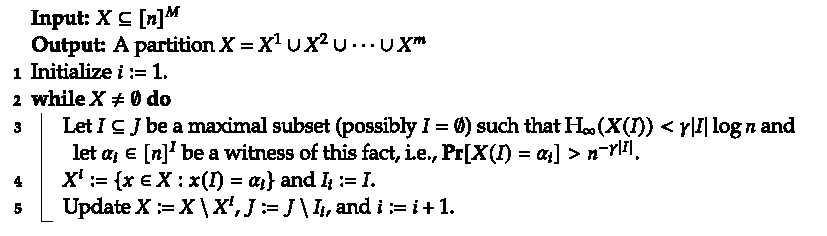
\includegraphics[width=\linewidth,height=0.78\textheight,keepaspectratio]{ccc2025-33-svg-03.pdf}\par




Item 1 is guaranteed by the construction of $X^{i}$ and $I_{i}$.\par




We prove Item 2 by contradiction.
Assume towards contradiction that $\bm{X}^{i}(J\setminus I_{i})$ is not $\gamma$-dense for some $i$.
By definition, there is a nonempty set $K\subseteq J\setminus I_{i}$ and $\beta\in[n]^{K}$ violating the min-entropy condition, namely,
$\operatorname*{\mathbf{Pr}}\left[\bm{X}(K)=\beta\right]>n^{-\gamma|K|}.$
Write $X^{\geq i}\stackrel{{\scriptstyle\mathsf{def}}}{{=}}\cup_{j\geq i}X^{i}$.
Then\par


\[\begin{gathered}
\operatorname*{\mathbf{Pr}}\left[\bm{X}^{\geq i}(I_{i}\cup K)=(\alpha_{i},\beta)\right]=\operatorname*{\mathbf{Pr}}\left[\bm{X}^{\geq i}(I_{i})=\alpha_{i}\right]\cdot\operatorname*{\mathbf{Pr}}\left[\bm{X}^{i}(K)=\beta\right]>n^{-\gamma|I_{i}|}\cdot n^{-\gamma|K|}=n^{-\gamma|I_{i}\cup K|},
\end{gathered}\]


where the first equality holds as $(\bm{X}^{\geq i}|\bm{X}^{\geq i}(I_{i})=\alpha_{i})=\bm{X}^{i}$.
However, this means at moment that $I_{i}$ is chosen,
the set $I_{i}\cup K\subseteq J$ also violates the min-entropy condition (witnessed by $(\alpha_{i},\beta)$), contradicting the maximality of $I_{i}$.\par




Finally, Item 3 is proved by straightforward calculation:\par


\[\begin{gathered}
\displaystyle D_{\infty}(\bm{X}^{i}(J\setminus I_{i})) \displaystyle=|J\setminus I_{i}|\log n-\log|X^{i}| \\
\displaystyle\leq(|J|\log n-|I_{i}|\log n)-\log\left(\left|X^{\geq i}\right|\cdot n^{-\gamma|I_{i}|}\right) \\
\displaystyle=(|J|\log n-\log|X|)-(1-\gamma)|I_{i}|\cdot\log n+\log\left(\frac{|X|}{\left|X^{\geq i}\right|}\right) \\
\displaystyle=D_{\infty}\Big{(}\bm{X}(J)\Big{)}-(1-\gamma)|I_{i}|\log n+\delta_{i}.\
\end{gathered}\]


$\blacktriangleleft$\par




\par




\end{document}
